\cleardoublepage
\chapter{Exact Algorithms for the $k$-Centre Problem}
\label{chap:algos}
%\lhead{Chapter \ref{chap:algos}. \emph{\nameref{chap:algos}}} % This is for the header

This chapter describes two possible algorithms that solve the \emph{$k$-centre} problem. The goal of this problem is to, given a set $N$ of $n$ points, find the subset of centroids of cardinality $k$ that minimises the farthest distance of a point in $N$ to its closest centroid. 

Both algorithms use an incremental branch-and-bound approach for implicit enumeration. The first algorithm is a naïve implementation of a branch-and-bound algorithm and uses simple loops over arrays for point location queries. The second algorithm builds and uses Delaunay triangulations to achieve more efficient point location queries. At the end of this chapter, these algorithms, as well as an implementation of the Integer Linear Programming formulation described in Section \ref{alg:ilp}, are experimentally tested in a set of benchmark instances.

\section{Naïve Branch-and-Bound}
\label{alg:bb}

One possible approach to this problem is to use a branch-and-bound method. Our approach is based on the wotk of \citet{incrementalcov} for solving a related $k$-centre problem. Their method describes algorithms to incrementally insert and remove centroids from a set of points, and update the centroid assignment only in the geometrical area surrounding the changed point. This method allows for small modifications on an already valid solution, and the techniques for updating the objective function upon insertion and removal of points can be used in an incremental branch-and-bound method to speed up the computation between branches, without having to calculate the full point assignment for every iteration of the algorithm, whilst still implicitly enumerating all possible combinations. 

To solve the problem incrementally, at each step of the recursive tree, one of the available points is considered. A decision is then taken of whether the point is a centroid or a non-centroid. According to which decision is taken, the objective function and the centroid assignment is updated accordingly. This is done until all the centroids have been chosen and a solution is found at the end of the branch. The best solution in all the branches is the optimal value for the \emph{$k$-centre} problem.

\subsection{Branching}
As stated above, branching the tree involves updating the assignment between new points and/or new centroids, as well as updating the objective function. The following procedures explain in detail how to do so.
\paragraph{Inserting a Centroid}
To insert a centroid $c$, the established non-centroids which are closer to $c$ than their current centroid must be checked, and change their assignment to $c$.
Since non-centroids only change assignment to centroids closer to them, inserting a centroid means that the objective function either decreases in value or stays the same.\\
After inserting a centroid, if the farthest non-centroid is reassigned, all non-centroids must be checked to see which one now maximises the objective function.
This step compares all non-centroids to the new centroid $c$, taking $\Theta(N)$ time. Figure \ref{fig:ncent} illustrates this operation.

\begin{figure}[!h]
\centering
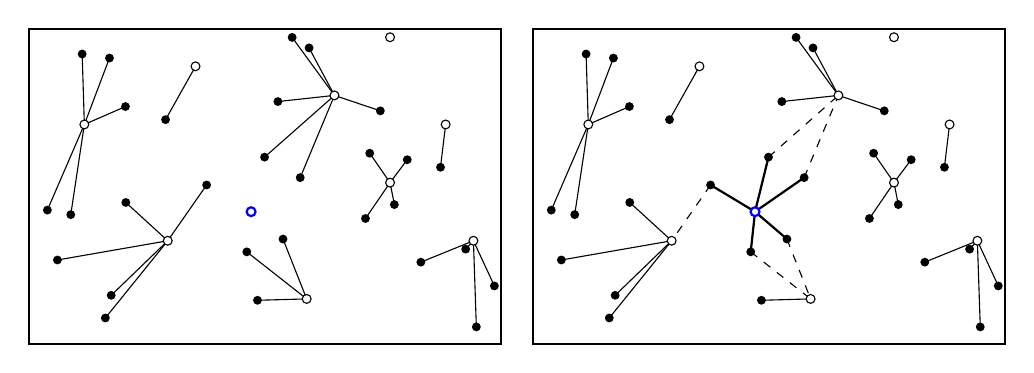
\begin{tikzpicture}[scale=0.4]
\draw [<->,thick] (0,0) rectangle (15,10) {};
\draw [-](7.261764705882353, 1.3796923076923076) -- (8.823529411764707, 1.4230769230769231);
\draw [-](10.690588235294118, 3.9763076923076923) -- (11.470588235294118, 5.115384615384615);
\draw [-](3.0697058823529413, 7.531076923076923) -- (1.7647058823529411, 6.961538461538462);
\draw [-](11.161764705882353, 7.393538461538461) -- (9.705882352941176, 7.884615384615385);
\draw [-](2.4308823529411763, 0.8175384615384615) -- (4.411764705882353, 3.269230769230769);
\draw [-](11.60735294117647, 4.418461538461538) -- (11.470588235294118, 5.115384615384615);
\draw [-](2.617058823529412, 1.5375384615384617) -- (4.411764705882353, 3.269230769230769);
\draw [-](8.617941176470588, 5.274153846153846) -- (9.705882352941176, 7.884615384615385);
\draw [-](0.5902941176470589, 4.243076923076923) -- (1.7647058823529411, 6.961538461538462);
\draw [-](1.695, 9.199076923076923) -- (1.7647058823529411, 6.961538461538462);
\draw [-](4.342941176470588, 7.114769230769231) -- (5.294117647058823, 8.807692307692308);
\draw [-](8.899411764705881, 9.392923076923077) -- (9.705882352941176, 7.884615384615385);
\draw [-](7.485882352941177, 5.924) -- (9.705882352941176, 7.884615384615385);
\draw [-](14.21029411764706, 0.5341538461538462) -- (14.117647058823529, 3.269230769230769);
\draw [-](14.78294117647059, 1.8356923076923077) -- (14.117647058823529, 3.269230769230769);
\draw [-](13.871470588235294, 3.0033846153846158) -- (14.117647058823529, 3.269230769230769);
\draw [-](1.333235294117647, 4.099076923076923) -- (1.7647058823529411, 6.961538461538462);
\draw [-](2.5623529411764707, 9.070769230769232) -- (1.7647058823529411, 6.961538461538462);
\draw [-](12.015882352941176, 5.842769230769231) -- (11.470588235294118, 5.115384615384615);
\draw [-](12.448235294117648, 2.5898461538461537) -- (14.117647058823529, 3.269230769230769);
\draw [-](0.909705882352941, 2.659076923076923) -- (4.411764705882353, 3.269230769230769);
\draw [-](3.0811764705882356, 4.485846153846154) -- (4.411764705882353, 3.269230769230769);
\draw [-](8.362058823529411, 9.726153846153846) -- (9.705882352941176, 7.884615384615385);
\draw [-](10.824705882352943, 6.048615384615385) -- (11.470588235294118, 5.115384615384615);
\draw [-](5.647058823529412, 5.040615384615384) -- (4.411764705882353, 3.269230769230769);
\draw [-](8.071764705882353, 3.3236923076923075) -- (8.823529411764707, 1.4230769230769231);
\draw [-](13.072058823529412, 5.602769230769231) -- (13.235294117647058, 6.961538461538462);
\draw [-](6.922058823529412, 2.917538461538462) -- (8.823529411764707, 1.4230769230769231);
\draw [-](7.909411764705883, 7.688923076923077) -- (9.705882352941176, 7.884615384615385);
\fill [white](1.7647058823529411, 6.961538461538462)circle(4pt);
\draw (1.7647058823529411, 6.961538461538462)circle(4pt);
\fill [white](4.411764705882353, 3.269230769230769)circle(4pt);
\draw (4.411764705882353, 3.269230769230769)circle(4pt);
\fill [white](5.294117647058823, 8.807692307692308)circle(4pt);
\draw (5.294117647058823, 8.807692307692308)circle(4pt);
\fill [white](8.823529411764707, 1.4230769230769231)circle(4pt);
\draw (8.823529411764707, 1.4230769230769231)circle(4pt);
\fill [white](9.705882352941176, 7.884615384615385)circle(4pt);
\draw (9.705882352941176, 7.884615384615385)circle(4pt);
\fill [white](11.470588235294118, 5.115384615384615)circle(4pt);
\draw (11.470588235294118, 5.115384615384615)circle(4pt);
\fill [white](11.470588235294118, 9.73076923076923)circle(4pt);
\draw (11.470588235294118, 9.73076923076923)circle(4pt);
\fill [white](13.235294117647058, 6.961538461538462)circle(4pt);
\draw (13.235294117647058, 6.961538461538462)circle(4pt);
\fill [white](14.117647058823529, 3.269230769230769)circle(4pt);
\draw (14.117647058823529, 3.269230769230769)circle(4pt);
\fill [white](7.0588235294117645, 4.1923076923076925)circle(4pt);
\draw [blue,thick](7.0588235294117645, 4.1923076923076925)circle(4pt);
\fill(7.261764705882353, 1.3796923076923076)circle(4pt);
\fill(10.690588235294118, 3.9763076923076923)circle(4pt);
\fill(3.0697058823529413, 7.531076923076923)circle(4pt);
\fill(11.161764705882353, 7.393538461538461)circle(4pt);
\fill(2.4308823529411763, 0.8175384615384615)circle(4pt);
\fill(11.60735294117647, 4.418461538461538)circle(4pt);
\fill(2.617058823529412, 1.5375384615384617)circle(4pt);
\fill(8.617941176470588, 5.274153846153846)circle(4pt);
\fill(0.5902941176470589, 4.243076923076923)circle(4pt);
\fill(1.695, 9.199076923076923)circle(4pt);
\fill(4.342941176470588, 7.114769230769231)circle(4pt);
\fill(8.899411764705881, 9.392923076923077)circle(4pt);
\fill(7.485882352941177, 5.924)circle(4pt);
\fill(14.21029411764706, 0.5341538461538462)circle(4pt);
\fill(14.78294117647059, 1.8356923076923077)circle(4pt);
\fill(13.871470588235294, 3.0033846153846158)circle(4pt);
\fill(1.333235294117647, 4.099076923076923)circle(4pt);
\fill(2.5623529411764707, 9.070769230769232)circle(4pt);
\fill(12.015882352941176, 5.842769230769231)circle(4pt);
\fill(12.448235294117648, 2.5898461538461537)circle(4pt);
\fill(0.909705882352941, 2.659076923076923)circle(4pt);
\fill(3.0811764705882356, 4.485846153846154)circle(4pt);
\fill(8.362058823529411, 9.726153846153846)circle(4pt);
\fill(10.824705882352943, 6.048615384615385)circle(4pt);
\fill(5.647058823529412, 5.040615384615384)circle(4pt);
\fill(8.071764705882353, 3.3236923076923075)circle(4pt);
\fill(13.072058823529412, 5.602769230769231)circle(4pt);
\fill(6.922058823529412, 2.917538461538462)circle(4pt);
\fill(7.909411764705883, 7.688923076923077)circle(4pt);
\begin{scope}[shift={(16,0)}]
\draw [<->,thick] (0,0) rectangle (15,10) {};
\draw [-](7.261764705882353, 1.3796923076923076) -- (8.823529411764707, 1.4230769230769231);
\draw [-](10.690588235294118, 3.9763076923076923) -- (11.470588235294118, 5.115384615384615);
\draw [-](3.0697058823529413, 7.531076923076923) -- (1.7647058823529411, 6.961538461538462);
\draw [-](11.161764705882353, 7.393538461538461) -- (9.705882352941176, 7.884615384615385);
\draw [-](2.4308823529411763, 0.8175384615384615) -- (4.411764705882353, 3.269230769230769);
\draw [-](11.60735294117647, 4.418461538461538) -- (11.470588235294118, 5.115384615384615);
\draw [-](2.617058823529412, 1.5375384615384617) -- (4.411764705882353, 3.269230769230769);
\draw [-,dashed](8.617941176470588, 5.274153846153846) -- (9.705882352941176, 7.884615384615385);
\draw [-](0.5902941176470589, 4.243076923076923) -- (1.7647058823529411, 6.961538461538462);
\draw [-](1.695, 9.199076923076923) -- (1.7647058823529411, 6.961538461538462);
\draw [-](4.342941176470588, 7.114769230769231) -- (5.294117647058823, 8.807692307692308);
\draw [-](8.899411764705881, 9.392923076923077) -- (9.705882352941176, 7.884615384615385);
\draw [-,dashed](7.485882352941177, 5.924) -- (9.705882352941176, 7.884615384615385);
\draw [-](14.21029411764706, 0.5341538461538462) -- (14.117647058823529, 3.269230769230769);
\draw [-](14.78294117647059, 1.8356923076923077) -- (14.117647058823529, 3.269230769230769);
\draw [-](13.871470588235294, 3.0033846153846158) -- (14.117647058823529, 3.269230769230769);
\draw [-](1.333235294117647, 4.099076923076923) -- (1.7647058823529411, 6.961538461538462);
\draw [-](2.5623529411764707, 9.070769230769232) -- (1.7647058823529411, 6.961538461538462);
\draw [-](12.015882352941176, 5.842769230769231) -- (11.470588235294118, 5.115384615384615);
\draw [-](12.448235294117648, 2.5898461538461537) -- (14.117647058823529, 3.269230769230769);
\draw [-](0.909705882352941, 2.659076923076923) -- (4.411764705882353, 3.269230769230769);
\draw [-](3.0811764705882356, 4.485846153846154) -- (4.411764705882353, 3.269230769230769);
\draw [-](8.362058823529411, 9.726153846153846) -- (9.705882352941176, 7.884615384615385);
\draw [-](10.824705882352943, 6.048615384615385) -- (11.470588235294118, 5.115384615384615);
\draw [-,dashed](5.647058823529412, 5.040615384615384) -- (4.411764705882353, 3.269230769230769);
\draw [-,dashed](8.071764705882353, 3.3236923076923075) -- (8.823529411764707, 1.4230769230769231);
\draw [-](13.072058823529412, 5.602769230769231) -- (13.235294117647058, 6.961538461538462);
\draw [-,dashed](6.922058823529412, 2.917538461538462) -- (8.823529411764707, 1.4230769230769231);
\draw [-](7.909411764705883, 7.688923076923077) -- (9.705882352941176, 7.884615384615385);
\draw [-,thick](8.617941176470588, 5.274153846153846) -- (7.0588235294117645, 4.1923076923076925);
\draw [-,thick](7.485882352941177, 5.924) -- (7.0588235294117645, 4.1923076923076925);
\draw [-,thick](5.647058823529412, 5.040615384615384) -- (7.0588235294117645, 4.1923076923076925);
\draw [-,thick](8.071764705882353, 3.3236923076923075) -- (7.0588235294117645, 4.1923076923076925);
\draw [-,thick](6.922058823529412, 2.917538461538462) -- (7.0588235294117645, 4.1923076923076925);
\fill [white](1.7647058823529411, 6.961538461538462)circle(4pt);
\draw (1.7647058823529411, 6.961538461538462)circle(4pt);
\fill [white](4.411764705882353, 3.269230769230769)circle(4pt);
\draw (4.411764705882353, 3.269230769230769)circle(4pt);
\fill [white](5.294117647058823, 8.807692307692308)circle(4pt);
\draw (5.294117647058823, 8.807692307692308)circle(4pt);
\fill [white](8.823529411764707, 1.4230769230769231)circle(4pt);
\draw (8.823529411764707, 1.4230769230769231)circle(4pt);
\fill [white](9.705882352941176, 7.884615384615385)circle(4pt);
\draw (9.705882352941176, 7.884615384615385)circle(4pt);
\fill [white](11.470588235294118, 5.115384615384615)circle(4pt);
\draw (11.470588235294118, 5.115384615384615)circle(4pt);
\fill [white](11.470588235294118, 9.73076923076923)circle(4pt);
\draw (11.470588235294118, 9.73076923076923)circle(4pt);
\fill [white](13.235294117647058, 6.961538461538462)circle(4pt);
\draw (13.235294117647058, 6.961538461538462)circle(4pt);
\fill [white](14.117647058823529, 3.269230769230769)circle(4pt);
\draw (14.117647058823529, 3.269230769230769)circle(4pt);
\fill [white](7.0588235294117645, 4.1923076923076925)circle(4pt);
\draw [blue,thick](7.0588235294117645, 4.1923076923076925)circle(4pt);
\fill(7.261764705882353, 1.3796923076923076)circle(4pt);
\fill(10.690588235294118, 3.9763076923076923)circle(4pt);
\fill(3.0697058823529413, 7.531076923076923)circle(4pt);
\fill(11.161764705882353, 7.393538461538461)circle(4pt);
\fill(2.4308823529411763, 0.8175384615384615)circle(4pt);
\fill(11.60735294117647, 4.418461538461538)circle(4pt);
\fill(2.617058823529412, 1.5375384615384617)circle(4pt);
\fill(8.617941176470588, 5.274153846153846)circle(4pt);
\fill(0.5902941176470589, 4.243076923076923)circle(4pt);
\fill(1.695, 9.199076923076923)circle(4pt);
\fill(4.342941176470588, 7.114769230769231)circle(4pt);
\fill(8.899411764705881, 9.392923076923077)circle(4pt);
\fill(7.485882352941177, 5.924)circle(4pt);
\fill(14.21029411764706, 0.5341538461538462)circle(4pt);
\fill(14.78294117647059, 1.8356923076923077)circle(4pt);
\fill(13.871470588235294, 3.0033846153846158)circle(4pt);
\fill(1.333235294117647, 4.099076923076923)circle(4pt);
\fill(2.5623529411764707, 9.070769230769232)circle(4pt);
\fill(12.015882352941176, 5.842769230769231)circle(4pt);
\fill(12.448235294117648, 2.5898461538461537)circle(4pt);
\fill(0.909705882352941, 2.659076923076923)circle(4pt);
\fill(3.0811764705882356, 4.485846153846154)circle(4pt);
\fill(8.362058823529411, 9.726153846153846)circle(4pt);
\fill(10.824705882352943, 6.048615384615385)circle(4pt);
\fill(5.647058823529412, 5.040615384615384)circle(4pt);
\fill(8.071764705882353, 3.3236923076923075)circle(4pt);
\fill(13.072058823529412, 5.602769230769231)circle(4pt);
\fill(6.922058823529412, 2.917538461538462)circle(4pt);
\fill(7.909411764705883, 7.688923076923077)circle(4pt);
\end{scope}
\end{tikzpicture}
\caption[Illustration of a centroid insertion.]{Illustration of a centroid insertion. The new point, in blue, changes the assignment of neighbouring points (in dashed lines), to connect to the new closest centroid.}
\label{fig:ncent}
\vspace{-5pt}
\end{figure}


\paragraph{Inserting a Non-Centroid}
Inserting a non-centroid $n$ only requires finding which of the current centroids is the closest to $n$. Updating the objective function is a matter of testing whether the distance between $n$ and its centroid is larger than the current maximum.
Inserting a non-centroid cannot produce a better objective function, since it either decreases or maintains the current value. 
This step compares the distance between point $n$ and all centroids, taking $\Theta(k)$ time. Figure \ref{fig:nncent} illustrates this step.

\begin{figure}[!h]
\centering
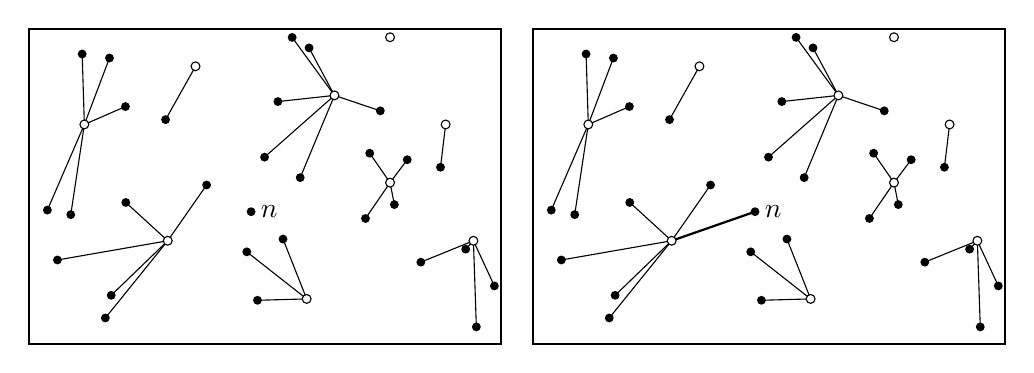
\begin{tikzpicture}[scale=0.4]
\draw [<->,thick] (0,0) rectangle (15,10) {};
\draw [-](7.261764705882353, 1.3796923076923076) -- (8.823529411764707, 1.4230769230769231);
\draw [-](10.690588235294118, 3.9763076923076923) -- (11.470588235294118, 5.115384615384615);
\draw [-](3.0697058823529413, 7.531076923076923) -- (1.7647058823529411, 6.961538461538462);
\draw [-](11.161764705882353, 7.393538461538461) -- (9.705882352941176, 7.884615384615385);
\draw [-](2.4308823529411763, 0.8175384615384615) -- (4.411764705882353, 3.269230769230769);
\draw [-](11.60735294117647, 4.418461538461538) -- (11.470588235294118, 5.115384615384615);
\draw [-](2.617058823529412, 1.5375384615384617) -- (4.411764705882353, 3.269230769230769);
\draw [-](8.617941176470588, 5.274153846153846) -- (9.705882352941176, 7.884615384615385);
\draw [-](0.5902941176470589, 4.243076923076923) -- (1.7647058823529411, 6.961538461538462);
\draw [-](1.695, 9.199076923076923) -- (1.7647058823529411, 6.961538461538462);
\draw [-](4.342941176470588, 7.114769230769231) -- (5.294117647058823, 8.807692307692308);
\draw [-](8.899411764705881, 9.392923076923077) -- (9.705882352941176, 7.884615384615385);
\draw [-](7.485882352941177, 5.924) -- (9.705882352941176, 7.884615384615385);
\draw [-](14.21029411764706, 0.5341538461538462) -- (14.117647058823529, 3.269230769230769);
\draw [-](14.78294117647059, 1.8356923076923077) -- (14.117647058823529, 3.269230769230769);
\draw [-](13.871470588235294, 3.0033846153846158) -- (14.117647058823529, 3.269230769230769);
\draw [-](1.333235294117647, 4.099076923076923) -- (1.7647058823529411, 6.961538461538462);
\draw [-](2.5623529411764707, 9.070769230769232) -- (1.7647058823529411, 6.961538461538462);
\draw [-](12.015882352941176, 5.842769230769231) -- (11.470588235294118, 5.115384615384615);
\draw [-](12.448235294117648, 2.5898461538461537) -- (14.117647058823529, 3.269230769230769);
\draw [-](0.909705882352941, 2.659076923076923) -- (4.411764705882353, 3.269230769230769);
\draw [-](3.0811764705882356, 4.485846153846154) -- (4.411764705882353, 3.269230769230769);
\draw [-](8.362058823529411, 9.726153846153846) -- (9.705882352941176, 7.884615384615385);
\draw [-](10.824705882352943, 6.048615384615385) -- (11.470588235294118, 5.115384615384615);
\draw [-](5.647058823529412, 5.040615384615384) -- (4.411764705882353, 3.269230769230769);
\draw [-](8.071764705882353, 3.3236923076923075) -- (8.823529411764707, 1.4230769230769231);
\draw [-](13.072058823529412, 5.602769230769231) -- (13.235294117647058, 6.961538461538462);
\draw [-](6.922058823529412, 2.917538461538462) -- (8.823529411764707, 1.4230769230769231);
\draw [-](7.909411764705883, 7.688923076923077) -- (9.705882352941176, 7.884615384615385);
\fill [white](1.7647058823529411, 6.961538461538462)circle(4pt);
\draw (1.7647058823529411, 6.961538461538462)circle(4pt);
\fill [white](4.411764705882353, 3.269230769230769)circle(4pt);
\draw (4.411764705882353, 3.269230769230769)circle(4pt);
\fill [white](5.294117647058823, 8.807692307692308)circle(4pt);
\draw (5.294117647058823, 8.807692307692308)circle(4pt);
\fill [white](8.823529411764707, 1.4230769230769231)circle(4pt);
\draw (8.823529411764707, 1.4230769230769231)circle(4pt);
\fill [white](9.705882352941176, 7.884615384615385)circle(4pt);
\draw (9.705882352941176, 7.884615384615385)circle(4pt);
\fill [white](11.470588235294118, 5.115384615384615)circle(4pt);
\draw (11.470588235294118, 5.115384615384615)circle(4pt);
\fill [white](11.470588235294118, 9.73076923076923)circle(4pt);
\draw (11.470588235294118, 9.73076923076923)circle(4pt);
\fill [white](13.235294117647058, 6.961538461538462)circle(4pt);
\draw (13.235294117647058, 6.961538461538462)circle(4pt);
\fill [white](14.117647058823529, 3.269230769230769)circle(4pt);
\draw (14.117647058823529, 3.269230769230769)circle(4pt);
\fill(7.0588235294117645, 4.1923076923076925)circle(4pt);
\fill(7.261764705882353, 1.3796923076923076)circle(4pt);
\fill(10.690588235294118, 3.9763076923076923)circle(4pt);
\fill(3.0697058823529413, 7.531076923076923)circle(4pt);
\fill(11.161764705882353, 7.393538461538461)circle(4pt);
\fill(2.4308823529411763, 0.8175384615384615)circle(4pt);
\fill(11.60735294117647, 4.418461538461538)circle(4pt);
\fill(2.617058823529412, 1.5375384615384617)circle(4pt);
\fill(8.617941176470588, 5.274153846153846)circle(4pt);
\fill(0.5902941176470589, 4.243076923076923)circle(4pt);
\fill(1.695, 9.199076923076923)circle(4pt);
\fill(4.342941176470588, 7.114769230769231)circle(4pt);
\fill(8.899411764705881, 9.392923076923077)circle(4pt);
\fill(7.485882352941177, 5.924)circle(4pt);
\fill(14.21029411764706, 0.5341538461538462)circle(4pt);
\fill(14.78294117647059, 1.8356923076923077)circle(4pt);
\fill(13.871470588235294, 3.0033846153846158)circle(4pt);
\fill(1.333235294117647, 4.099076923076923)circle(4pt);
\fill(2.5623529411764707, 9.070769230769232)circle(4pt);
\fill(12.015882352941176, 5.842769230769231)circle(4pt);
\fill(12.448235294117648, 2.5898461538461537)circle(4pt);
\fill(0.909705882352941, 2.659076923076923)circle(4pt);
\fill(3.0811764705882356, 4.485846153846154)circle(4pt);
\fill(8.362058823529411, 9.726153846153846)circle(4pt);
\fill(10.824705882352943, 6.048615384615385)circle(4pt);
\fill(5.647058823529412, 5.040615384615384)circle(4pt);
\fill(8.071764705882353, 3.3236923076923075)circle(4pt);
\fill(13.072058823529412, 5.602769230769231)circle(4pt);
\fill(6.922058823529412, 2.917538461538462)circle(4pt);
\fill(7.909411764705883, 7.688923076923077)circle(4pt);
\node at (7.0588235294117645, 4.1923076923076925)[right] {$n$};
\begin{scope}[shift={(16,0)}]
\draw [<->,thick] (0,0) rectangle (15,10) {};
\draw [-](7.261764705882353, 1.3796923076923076) -- (8.823529411764707, 1.4230769230769231);
\draw [-](10.690588235294118, 3.9763076923076923) -- (11.470588235294118, 5.115384615384615);
\draw [-](3.0697058823529413, 7.531076923076923) -- (1.7647058823529411, 6.961538461538462);
\draw [-](11.161764705882353, 7.393538461538461) -- (9.705882352941176, 7.884615384615385);
\draw [-](2.4308823529411763, 0.8175384615384615) -- (4.411764705882353, 3.269230769230769);
\draw [-](11.60735294117647, 4.418461538461538) -- (11.470588235294118, 5.115384615384615);
\draw [-](2.617058823529412, 1.5375384615384617) -- (4.411764705882353, 3.269230769230769);
\draw [-](8.617941176470588, 5.274153846153846) -- (9.705882352941176, 7.884615384615385);
\draw [-](0.5902941176470589, 4.243076923076923) -- (1.7647058823529411, 6.961538461538462);
\draw [-](1.695, 9.199076923076923) -- (1.7647058823529411, 6.961538461538462);
\draw [-](4.342941176470588, 7.114769230769231) -- (5.294117647058823, 8.807692307692308);
\draw [-](8.899411764705881, 9.392923076923077) -- (9.705882352941176, 7.884615384615385);
\draw [-](7.485882352941177, 5.924) -- (9.705882352941176, 7.884615384615385);
\draw [-](14.21029411764706, 0.5341538461538462) -- (14.117647058823529, 3.269230769230769);
\draw [-](14.78294117647059, 1.8356923076923077) -- (14.117647058823529, 3.269230769230769);
\draw [-](13.871470588235294, 3.0033846153846158) -- (14.117647058823529, 3.269230769230769);
\draw [-](1.333235294117647, 4.099076923076923) -- (1.7647058823529411, 6.961538461538462);
\draw [-](2.5623529411764707, 9.070769230769232) -- (1.7647058823529411, 6.961538461538462);
\draw [-](12.015882352941176, 5.842769230769231) -- (11.470588235294118, 5.115384615384615);
\draw [-](12.448235294117648, 2.5898461538461537) -- (14.117647058823529, 3.269230769230769);
\draw [-](0.909705882352941, 2.659076923076923) -- (4.411764705882353, 3.269230769230769);
\draw [-](3.0811764705882356, 4.485846153846154) -- (4.411764705882353, 3.269230769230769);
\draw [-](8.362058823529411, 9.726153846153846) -- (9.705882352941176, 7.884615384615385);
\draw [-](10.824705882352943, 6.048615384615385) -- (11.470588235294118, 5.115384615384615);
\draw [-](5.647058823529412, 5.040615384615384) -- (4.411764705882353, 3.269230769230769);
\draw [-](8.071764705882353, 3.3236923076923075) -- (8.823529411764707, 1.4230769230769231);
\draw [-](13.072058823529412, 5.602769230769231) -- (13.235294117647058, 6.961538461538462);
\draw [-](6.922058823529412, 2.917538461538462) -- (8.823529411764707, 1.4230769230769231);
\draw [-](7.909411764705883, 7.688923076923077) -- (9.705882352941176, 7.884615384615385);
\draw [-,thick](7.0588235294117645, 4.1923076923076925) -- (4.411764705882353, 3.269230769230769);
\fill [white](1.7647058823529411, 6.961538461538462)circle(4pt);
\draw (1.7647058823529411, 6.961538461538462)circle(4pt);
\fill [white](4.411764705882353, 3.269230769230769)circle(4pt);
\draw (4.411764705882353, 3.269230769230769)circle(4pt);
\fill [white](5.294117647058823, 8.807692307692308)circle(4pt);
\draw (5.294117647058823, 8.807692307692308)circle(4pt);
\fill [white](8.823529411764707, 1.4230769230769231)circle(4pt);
\draw (8.823529411764707, 1.4230769230769231)circle(4pt);
\fill [white](9.705882352941176, 7.884615384615385)circle(4pt);
\draw (9.705882352941176, 7.884615384615385)circle(4pt);
\fill [white](11.470588235294118, 5.115384615384615)circle(4pt);
\draw (11.470588235294118, 5.115384615384615)circle(4pt);
\fill [white](11.470588235294118, 9.73076923076923)circle(4pt);
\draw (11.470588235294118, 9.73076923076923)circle(4pt);
\fill [white](13.235294117647058, 6.961538461538462)circle(4pt);
\draw (13.235294117647058, 6.961538461538462)circle(4pt);
\fill [white](14.117647058823529, 3.269230769230769)circle(4pt);
\draw (14.117647058823529, 3.269230769230769)circle(4pt);
\fill (7.0588235294117645, 4.1923076923076925)circle(4pt);
\fill(7.261764705882353, 1.3796923076923076)circle(4pt);
\fill(10.690588235294118, 3.9763076923076923)circle(4pt);
\fill(3.0697058823529413, 7.531076923076923)circle(4pt);
\fill(11.161764705882353, 7.393538461538461)circle(4pt);
\fill(2.4308823529411763, 0.8175384615384615)circle(4pt);
\fill(11.60735294117647, 4.418461538461538)circle(4pt);
\fill(2.617058823529412, 1.5375384615384617)circle(4pt);
\fill(8.617941176470588, 5.274153846153846)circle(4pt);
\fill(0.5902941176470589, 4.243076923076923)circle(4pt);
\fill(1.695, 9.199076923076923)circle(4pt);
\fill(4.342941176470588, 7.114769230769231)circle(4pt);
\fill(8.899411764705881, 9.392923076923077)circle(4pt);
\fill(7.485882352941177, 5.924)circle(4pt);
\fill(14.21029411764706, 0.5341538461538462)circle(4pt);
\fill(14.78294117647059, 1.8356923076923077)circle(4pt);
\fill(13.871470588235294, 3.0033846153846158)circle(4pt);
\fill(1.333235294117647, 4.099076923076923)circle(4pt);
\fill(2.5623529411764707, 9.070769230769232)circle(4pt);
\fill(12.015882352941176, 5.842769230769231)circle(4pt);
\fill(12.448235294117648, 2.5898461538461537)circle(4pt);
\fill(0.909705882352941, 2.659076923076923)circle(4pt);
\fill(3.0811764705882356, 4.485846153846154)circle(4pt);
\fill(8.362058823529411, 9.726153846153846)circle(4pt);
\fill(10.824705882352943, 6.048615384615385)circle(4pt);
\fill(5.647058823529412, 5.040615384615384)circle(4pt);
\fill(8.071764705882353, 3.3236923076923075)circle(4pt);
\fill(13.072058823529412, 5.602769230769231)circle(4pt);
\fill(6.922058823529412, 2.917538461538462)circle(4pt);
\fill(7.909411764705883, 7.688923076923077)circle(4pt);
\node at (7.0588235294117645, 4.1923076923076925)[right] {$n$};
\end{scope}
\end{tikzpicture}
\caption[Illustration of a non-centroid insertion]{Illustration of a non-centroid insertion. The new non-centroid, $n$, is assigned to the closest centroid.}
\label{fig:nncent}
\end{figure}


\paragraph{}
After a branch is fully calculated, it is necessary to backtrack to the parent state, either by removing a centroid, or a non-centroid.

\paragraph{Removing a Centroid}
Removing a centroid $c$ means redistributing the values assigned to $c$ to their respective closest centroids in the remaining set. \\
The value function either increases or maintains, since the distance for all points previously assigned to $c$ increases, potentially above the current value for the objective function.
Removing a centroid $c$ means comparing all non-centroids assigned to $c$ to all the other centroids. This step takes $\Theta(NK)$ time to execute. Alternatively, if the assignment state is saved before inserting the centroid, recovering it requires only retrieving the state, which means, in the worst and best cases copying an array of size $N$, which takes $\Theta(N)$ time at the expense of additional $\Theta(N)$ memory space. Figure \ref{fig:rcent} illustrates this step.

\begin{figure}[H]
\centering
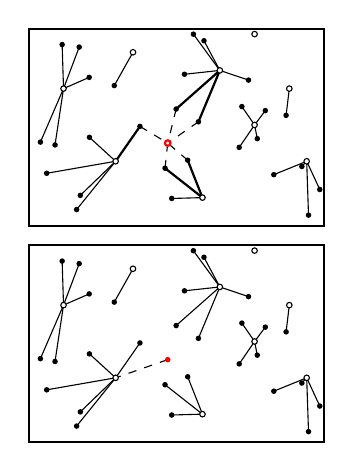
\begin{tikzpicture}[scale=0.25]
\begin{scope}[shift={(0,0)}]\draw [<->,thick] (0,0) rectangle (15,10) {};
\draw [-](7.261764705882353, 1.3796923076923076) -- (8.823529411764707, 1.4230769230769231);
\draw [-](10.690588235294118, 3.9763076923076923) -- (11.470588235294118, 5.115384615384615);
\draw [-](3.0697058823529413, 7.531076923076923) -- (1.7647058823529411, 6.961538461538462);
\draw [-](11.161764705882353, 7.393538461538461) -- (9.705882352941176, 7.884615384615385);
\draw [-](2.4308823529411763, 0.8175384615384615) -- (4.411764705882353, 3.269230769230769);
\draw [-](11.60735294117647, 4.418461538461538) -- (11.470588235294118, 5.115384615384615);
\draw [-](2.617058823529412, 1.5375384615384617) -- (4.411764705882353, 3.269230769230769);
\draw [-,thick](8.617941176470588, 5.274153846153846) -- (9.705882352941176, 7.884615384615385);
\draw [-](0.5902941176470589, 4.243076923076923) -- (1.7647058823529411, 6.961538461538462);
\draw [-](1.695, 9.199076923076923) -- (1.7647058823529411, 6.961538461538462);
\draw [-](4.342941176470588, 7.114769230769231) -- (5.294117647058823, 8.807692307692308);
\draw [-](8.899411764705881, 9.392923076923077) -- (9.705882352941176, 7.884615384615385);
\draw [-,thick](7.485882352941177, 5.924) -- (9.705882352941176, 7.884615384615385);
\draw [-](14.21029411764706, 0.5341538461538462) -- (14.117647058823529, 3.269230769230769);
\draw [-](14.78294117647059, 1.8356923076923077) -- (14.117647058823529, 3.269230769230769);
\draw [-](13.871470588235294, 3.0033846153846158) -- (14.117647058823529, 3.269230769230769);
\draw [-](1.333235294117647, 4.099076923076923) -- (1.7647058823529411, 6.961538461538462);
\draw [-](2.5623529411764707, 9.070769230769232) -- (1.7647058823529411, 6.961538461538462);
\draw [-](12.015882352941176, 5.842769230769231) -- (11.470588235294118, 5.115384615384615);
\draw [-](12.448235294117648, 2.5898461538461537) -- (14.117647058823529, 3.269230769230769);
\draw [-](0.909705882352941, 2.659076923076923) -- (4.411764705882353, 3.269230769230769);
\draw [-](3.0811764705882356, 4.485846153846154) -- (4.411764705882353, 3.269230769230769);
\draw [-](8.362058823529411, 9.726153846153846) -- (9.705882352941176, 7.884615384615385);
\draw [-](10.824705882352943, 6.048615384615385) -- (11.470588235294118, 5.115384615384615);
\draw [-,thick](5.647058823529412, 5.040615384615384) -- (4.411764705882353, 3.269230769230769);
\draw [-,thick](8.071764705882353, 3.3236923076923075) -- (8.823529411764707, 1.4230769230769231);
\draw [-](13.072058823529412, 5.602769230769231) -- (13.235294117647058, 6.961538461538462);
\draw [-,thick](6.922058823529412, 2.917538461538462) -- (8.823529411764707, 1.4230769230769231);
\draw [-](7.909411764705883, 7.688923076923077) -- (9.705882352941176, 7.884615384615385);
\draw [-,dashed](8.617941176470588, 5.274153846153846) -- (7.0588235294117645, 4.1923076923076925);
\draw [-,dashed](7.485882352941177, 5.924) -- (7.0588235294117645, 4.1923076923076925);
\draw [-,dashed](5.647058823529412, 5.040615384615384) -- (7.0588235294117645, 4.1923076923076925);
\draw [-,dashed](8.071764705882353, 3.3236923076923075) -- (7.0588235294117645, 4.1923076923076925);
\draw [-,dashed](6.922058823529412, 2.917538461538462) -- (7.0588235294117645, 4.1923076923076925);
\fill [white](1.7647058823529411, 6.961538461538462)circle(4pt);
\draw (1.7647058823529411, 6.961538461538462)circle(4pt);
\fill [white](4.411764705882353, 3.269230769230769)circle(4pt);
\draw (4.411764705882353, 3.269230769230769)circle(4pt);
\fill [white](5.294117647058823, 8.807692307692308)circle(4pt);
\draw (5.294117647058823, 8.807692307692308)circle(4pt);
\fill [white](8.823529411764707, 1.4230769230769231)circle(4pt);
\draw (8.823529411764707, 1.4230769230769231)circle(4pt);
\fill [white](9.705882352941176, 7.884615384615385)circle(4pt);
\draw (9.705882352941176, 7.884615384615385)circle(4pt);
\fill [white](11.470588235294118, 5.115384615384615)circle(4pt);
\draw (11.470588235294118, 5.115384615384615)circle(4pt);
\fill [white](11.470588235294118, 9.73076923076923)circle(4pt);
\draw (11.470588235294118, 9.73076923076923)circle(4pt);
\fill [white](13.235294117647058, 6.961538461538462)circle(4pt);
\draw (13.235294117647058, 6.961538461538462)circle(4pt);
\fill [white](14.117647058823529, 3.269230769230769)circle(4pt);
\draw (14.117647058823529, 3.269230769230769)circle(4pt);
\fill [white](7.0588235294117645, 4.1923076923076925)circle(4pt);
\draw [red,thick](7.0588235294117645, 4.1923076923076925)circle(4pt);
\fill(7.261764705882353, 1.3796923076923076)circle(4pt);
\fill(10.690588235294118, 3.9763076923076923)circle(4pt);
\fill(3.0697058823529413, 7.531076923076923)circle(4pt);
\fill(11.161764705882353, 7.393538461538461)circle(4pt);
\fill(2.4308823529411763, 0.8175384615384615)circle(4pt);
\fill(11.60735294117647, 4.418461538461538)circle(4pt);
\fill(2.617058823529412, 1.5375384615384617)circle(4pt);
\fill(8.617941176470588, 5.274153846153846)circle(4pt);
\fill(0.5902941176470589, 4.243076923076923)circle(4pt);
\fill(1.695, 9.199076923076923)circle(4pt);
\fill(4.342941176470588, 7.114769230769231)circle(4pt);
\fill(8.899411764705881, 9.392923076923077)circle(4pt);
\fill(7.485882352941177, 5.924)circle(4pt);
\fill(14.21029411764706, 0.5341538461538462)circle(4pt);
\fill(14.78294117647059, 1.8356923076923077)circle(4pt);
\fill(13.871470588235294, 3.0033846153846158)circle(4pt);
\fill(1.333235294117647, 4.099076923076923)circle(4pt);
\fill(2.5623529411764707, 9.070769230769232)circle(4pt);
\fill(12.015882352941176, 5.842769230769231)circle(4pt);
\fill(12.448235294117648, 2.5898461538461537)circle(4pt);
\fill(0.909705882352941, 2.659076923076923)circle(4pt);
\fill(3.0811764705882356, 4.485846153846154)circle(4pt);
\fill(8.362058823529411, 9.726153846153846)circle(4pt);
\fill(10.824705882352943, 6.048615384615385)circle(4pt);
\fill(5.647058823529412, 5.040615384615384)circle(4pt);
\fill(8.071764705882353, 3.3236923076923075)circle(4pt);
\fill(13.072058823529412, 5.602769230769231)circle(4pt);
\fill(6.922058823529412, 2.917538461538462)circle(4pt);
\fill(7.909411764705883, 7.688923076923077)circle(4pt);
\begin{scope}[shift={(0,-11)}]


\draw [<->,thick] (0,0) rectangle (15,10) {};
\draw [-](7.261764705882353, 1.3796923076923076) -- (8.823529411764707, 1.4230769230769231);
\draw [-](10.690588235294118, 3.9763076923076923) -- (11.470588235294118, 5.115384615384615);
\draw [-](3.0697058823529413, 7.531076923076923) -- (1.7647058823529411, 6.961538461538462);
\draw [-](11.161764705882353, 7.393538461538461) -- (9.705882352941176, 7.884615384615385);
\draw [-](2.4308823529411763, 0.8175384615384615) -- (4.411764705882353, 3.269230769230769);
\draw [-](11.60735294117647, 4.418461538461538) -- (11.470588235294118, 5.115384615384615);
\draw [-](2.617058823529412, 1.5375384615384617) -- (4.411764705882353, 3.269230769230769);
\draw [-](8.617941176470588, 5.274153846153846) -- (9.705882352941176, 7.884615384615385);
\draw [-](0.5902941176470589, 4.243076923076923) -- (1.7647058823529411, 6.961538461538462);
\draw [-](1.695, 9.199076923076923) -- (1.7647058823529411, 6.961538461538462);
\draw [-](4.342941176470588, 7.114769230769231) -- (5.294117647058823, 8.807692307692308);
\draw [-](8.899411764705881, 9.392923076923077) -- (9.705882352941176, 7.884615384615385);
\draw [-](7.485882352941177, 5.924) -- (9.705882352941176, 7.884615384615385);
\draw [-](14.21029411764706, 0.5341538461538462) -- (14.117647058823529, 3.269230769230769);
\draw [-](14.78294117647059, 1.8356923076923077) -- (14.117647058823529, 3.269230769230769);
\draw [-](13.871470588235294, 3.0033846153846158) -- (14.117647058823529, 3.269230769230769);
\draw [-](1.333235294117647, 4.099076923076923) -- (1.7647058823529411, 6.961538461538462);
\draw [-](2.5623529411764707, 9.070769230769232) -- (1.7647058823529411, 6.961538461538462);
\draw [-](12.015882352941176, 5.842769230769231) -- (11.470588235294118, 5.115384615384615);
\draw [-](12.448235294117648, 2.5898461538461537) -- (14.117647058823529, 3.269230769230769);
\draw [-](0.909705882352941, 2.659076923076923) -- (4.411764705882353, 3.269230769230769);
\draw [-](3.0811764705882356, 4.485846153846154) -- (4.411764705882353, 3.269230769230769);
\draw [-](8.362058823529411, 9.726153846153846) -- (9.705882352941176, 7.884615384615385);
\draw [-](10.824705882352943, 6.048615384615385) -- (11.470588235294118, 5.115384615384615);
\draw [-](5.647058823529412, 5.040615384615384) -- (4.411764705882353, 3.269230769230769);
\draw [-](8.071764705882353, 3.3236923076923075) -- (8.823529411764707, 1.4230769230769231);
\draw [-](13.072058823529412, 5.602769230769231) -- (13.235294117647058, 6.961538461538462);
\draw [-](6.922058823529412, 2.917538461538462) -- (8.823529411764707, 1.4230769230769231);
\draw [-](7.909411764705883, 7.688923076923077) -- (9.705882352941176, 7.884615384615385);
\draw [-,dashed](7.0588235294117645, 4.1923076923076925) -- (4.411764705882353, 3.269230769230769);
\fill [white](1.7647058823529411, 6.961538461538462)circle(4pt);
\draw (1.7647058823529411, 6.961538461538462)circle(4pt);
\fill [white](4.411764705882353, 3.269230769230769)circle(4pt);
\draw (4.411764705882353, 3.269230769230769)circle(4pt);
\fill [white](5.294117647058823, 8.807692307692308)circle(4pt);
\draw (5.294117647058823, 8.807692307692308)circle(4pt);
\fill [white](8.823529411764707, 1.4230769230769231)circle(4pt);
\draw (8.823529411764707, 1.4230769230769231)circle(4pt);
\fill [white](9.705882352941176, 7.884615384615385)circle(4pt);
\draw (9.705882352941176, 7.884615384615385)circle(4pt);
\fill [white](11.470588235294118, 5.115384615384615)circle(4pt);
\draw (11.470588235294118, 5.115384615384615)circle(4pt);
\fill [white](11.470588235294118, 9.73076923076923)circle(4pt);
\draw (11.470588235294118, 9.73076923076923)circle(4pt);
\fill [white](13.235294117647058, 6.961538461538462)circle(4pt);
\draw (13.235294117647058, 6.961538461538462)circle(4pt);
\fill [white](14.117647058823529, 3.269230769230769)circle(4pt);
\draw (14.117647058823529, 3.269230769230769)circle(4pt);
\fill [red](7.0588235294117645, 4.1923076923076925)circle(4pt);
\fill(7.261764705882353, 1.3796923076923076)circle(4pt);
\fill(10.690588235294118, 3.9763076923076923)circle(4pt);
\fill(3.0697058823529413, 7.531076923076923)circle(4pt);
\fill(11.161764705882353, 7.393538461538461)circle(4pt);
\fill(2.4308823529411763, 0.8175384615384615)circle(4pt);
\fill(11.60735294117647, 4.418461538461538)circle(4pt);
\fill(2.617058823529412, 1.5375384615384617)circle(4pt);
\fill(8.617941176470588, 5.274153846153846)circle(4pt);
\fill(0.5902941176470589, 4.243076923076923)circle(4pt);
\fill(1.695, 9.199076923076923)circle(4pt);
\fill(4.342941176470588, 7.114769230769231)circle(4pt);
\fill(8.899411764705881, 9.392923076923077)circle(4pt);
\fill(7.485882352941177, 5.924)circle(4pt);
\fill(14.21029411764706, 0.5341538461538462)circle(4pt);
\fill(14.78294117647059, 1.8356923076923077)circle(4pt);
\fill(13.871470588235294, 3.0033846153846158)circle(4pt);
\fill(1.333235294117647, 4.099076923076923)circle(4pt);
\fill(2.5623529411764707, 9.070769230769232)circle(4pt);
\fill(12.015882352941176, 5.842769230769231)circle(4pt);
\fill(12.448235294117648, 2.5898461538461537)circle(4pt);
\fill(0.909705882352941, 2.659076923076923)circle(4pt);
\fill(3.0811764705882356, 4.485846153846154)circle(4pt);
\fill(8.362058823529411, 9.726153846153846)circle(4pt);
\fill(10.824705882352943, 6.048615384615385)circle(4pt);
\fill(5.647058823529412, 5.040615384615384)circle(4pt);
\fill(8.071764705882353, 3.3236923076923075)circle(4pt);
\fill(13.072058823529412, 5.602769230769231)circle(4pt);
\fill(6.922058823529412, 2.917538461538462)circle(4pt);
\fill(7.909411764705883, 7.688923076923077)circle(4pt);
\end{scope}
\end{scope}
\end{tikzpicture}
\end{figure}


\paragraph{Removing a Non-Centroid}
In order to remove a non-centroid $n$, we only need to update the objective function. If point $n$ maximises the objective function, the second farthest point from its centroid, the new maximiser, must be found.
Removing a non-centroid can either decrease or maintain the value of the objective function.
Removing a non-centroid $n$ means that the next farthest point from its centroid must be found. This can be done by checking all distances between the non-centroids and their respective centroids, taking $\Theta(N)$ time. Alternatively, one can save the previous value for the objective function, as well as the maximiser. Retrieving the previous value can be done in $\mathcal{O}(1)$ time at the expense of additional $\Theta(1)$ memory space. Figure \ref{fig:rncent} illustrates this step.

\begin{figure}[!h]
\centering
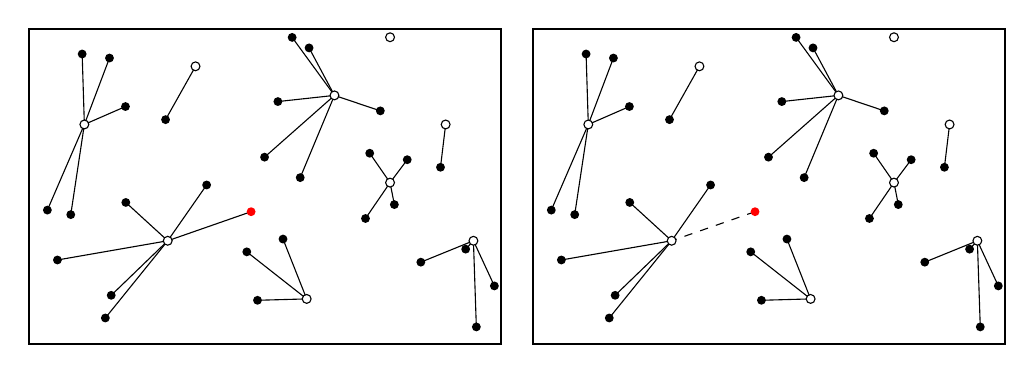
\begin{tikzpicture}[scale=0.4]
\draw [<->,thick] (0,0) rectangle (15,10) {};
\draw [-](7.261764705882353, 1.3796923076923076) -- (8.823529411764707, 1.4230769230769231);
\draw [-](10.690588235294118, 3.9763076923076923) -- (11.470588235294118, 5.115384615384615);
\draw [-](3.0697058823529413, 7.531076923076923) -- (1.7647058823529411, 6.961538461538462);
\draw [-](11.161764705882353, 7.393538461538461) -- (9.705882352941176, 7.884615384615385);
\draw [-](2.4308823529411763, 0.8175384615384615) -- (4.411764705882353, 3.269230769230769);
\draw [-](11.60735294117647, 4.418461538461538) -- (11.470588235294118, 5.115384615384615);
\draw [-](2.617058823529412, 1.5375384615384617) -- (4.411764705882353, 3.269230769230769);
\draw [-](8.617941176470588, 5.274153846153846) -- (9.705882352941176, 7.884615384615385);
\draw [-](0.5902941176470589, 4.243076923076923) -- (1.7647058823529411, 6.961538461538462);
\draw [-](1.695, 9.199076923076923) -- (1.7647058823529411, 6.961538461538462);
\draw [-](4.342941176470588, 7.114769230769231) -- (5.294117647058823, 8.807692307692308);
\draw [-](8.899411764705881, 9.392923076923077) -- (9.705882352941176, 7.884615384615385);
\draw [-](7.485882352941177, 5.924) -- (9.705882352941176, 7.884615384615385);
\draw [-](14.21029411764706, 0.5341538461538462) -- (14.117647058823529, 3.269230769230769);
\draw [-](14.78294117647059, 1.8356923076923077) -- (14.117647058823529, 3.269230769230769);
\draw [-](13.871470588235294, 3.0033846153846158) -- (14.117647058823529, 3.269230769230769);
\draw [-](1.333235294117647, 4.099076923076923) -- (1.7647058823529411, 6.961538461538462);
\draw [-](2.5623529411764707, 9.070769230769232) -- (1.7647058823529411, 6.961538461538462);
\draw [-](12.015882352941176, 5.842769230769231) -- (11.470588235294118, 5.115384615384615);
\draw [-](12.448235294117648, 2.5898461538461537) -- (14.117647058823529, 3.269230769230769);
\draw [-](0.909705882352941, 2.659076923076923) -- (4.411764705882353, 3.269230769230769);
\draw [-](3.0811764705882356, 4.485846153846154) -- (4.411764705882353, 3.269230769230769);
\draw [-](8.362058823529411, 9.726153846153846) -- (9.705882352941176, 7.884615384615385);
\draw [-](10.824705882352943, 6.048615384615385) -- (11.470588235294118, 5.115384615384615);
\draw [-](5.647058823529412, 5.040615384615384) -- (4.411764705882353, 3.269230769230769);
\draw [-](8.071764705882353, 3.3236923076923075) -- (8.823529411764707, 1.4230769230769231);
\draw [-](13.072058823529412, 5.602769230769231) -- (13.235294117647058, 6.961538461538462);
\draw [-](6.922058823529412, 2.917538461538462) -- (8.823529411764707, 1.4230769230769231);
\draw [-](7.909411764705883, 7.688923076923077) -- (9.705882352941176, 7.884615384615385);
\draw [-](7.0588235294117645, 4.1923076923076925) -- (4.411764705882353, 3.269230769230769);
\fill [white](1.7647058823529411, 6.961538461538462)circle(4pt);
\draw (1.7647058823529411, 6.961538461538462)circle(4pt);
\fill [white](4.411764705882353, 3.269230769230769)circle(4pt);
\draw (4.411764705882353, 3.269230769230769)circle(4pt);
\fill [white](5.294117647058823, 8.807692307692308)circle(4pt);
\draw (5.294117647058823, 8.807692307692308)circle(4pt);
\fill [white](8.823529411764707, 1.4230769230769231)circle(4pt);
\draw (8.823529411764707, 1.4230769230769231)circle(4pt);
\fill [white](9.705882352941176, 7.884615384615385)circle(4pt);
\draw (9.705882352941176, 7.884615384615385)circle(4pt);
\fill [white](11.470588235294118, 5.115384615384615)circle(4pt);
\draw (11.470588235294118, 5.115384615384615)circle(4pt);
\fill [white](11.470588235294118, 9.73076923076923)circle(4pt);
\draw (11.470588235294118, 9.73076923076923)circle(4pt);
\fill [white](13.235294117647058, 6.961538461538462)circle(4pt);
\draw (13.235294117647058, 6.961538461538462)circle(4pt);
\fill [white](14.117647058823529, 3.269230769230769)circle(4pt);
\draw (14.117647058823529, 3.269230769230769)circle(4pt);
\fill [red](7.0588235294117645, 4.1923076923076925)circle(4pt);
\fill(7.261764705882353, 1.3796923076923076)circle(4pt);
\fill(10.690588235294118, 3.9763076923076923)circle(4pt);
\fill(3.0697058823529413, 7.531076923076923)circle(4pt);
\fill(11.161764705882353, 7.393538461538461)circle(4pt);
\fill(2.4308823529411763, 0.8175384615384615)circle(4pt);
\fill(11.60735294117647, 4.418461538461538)circle(4pt);
\fill(2.617058823529412, 1.5375384615384617)circle(4pt);
\fill(8.617941176470588, 5.274153846153846)circle(4pt);
\fill(0.5902941176470589, 4.243076923076923)circle(4pt);
\fill(1.695, 9.199076923076923)circle(4pt);
\fill(4.342941176470588, 7.114769230769231)circle(4pt);
\fill(8.899411764705881, 9.392923076923077)circle(4pt);
\fill(7.485882352941177, 5.924)circle(4pt);
\fill(14.21029411764706, 0.5341538461538462)circle(4pt);
\fill(14.78294117647059, 1.8356923076923077)circle(4pt);
\fill(13.871470588235294, 3.0033846153846158)circle(4pt);
\fill(1.333235294117647, 4.099076923076923)circle(4pt);
\fill(2.5623529411764707, 9.070769230769232)circle(4pt);
\fill(12.015882352941176, 5.842769230769231)circle(4pt);
\fill(12.448235294117648, 2.5898461538461537)circle(4pt);
\fill(0.909705882352941, 2.659076923076923)circle(4pt);
\fill(3.0811764705882356, 4.485846153846154)circle(4pt);
\fill(8.362058823529411, 9.726153846153846)circle(4pt);
\fill(10.824705882352943, 6.048615384615385)circle(4pt);
\fill(5.647058823529412, 5.040615384615384)circle(4pt);
\fill(8.071764705882353, 3.3236923076923075)circle(4pt);
\fill(13.072058823529412, 5.602769230769231)circle(4pt);
\fill(6.922058823529412, 2.917538461538462)circle(4pt);
\fill(7.909411764705883, 7.688923076923077)circle(4pt);
\begin{scope}[shift={(16,0)}]
\draw [<->,thick] (0,0) rectangle (15,10) {};
\draw [-](7.261764705882353, 1.3796923076923076) -- (8.823529411764707, 1.4230769230769231);
\draw [-](10.690588235294118, 3.9763076923076923) -- (11.470588235294118, 5.115384615384615);
\draw [-](3.0697058823529413, 7.531076923076923) -- (1.7647058823529411, 6.961538461538462);
\draw [-](11.161764705882353, 7.393538461538461) -- (9.705882352941176, 7.884615384615385);
\draw [-](2.4308823529411763, 0.8175384615384615) -- (4.411764705882353, 3.269230769230769);
\draw [-](11.60735294117647, 4.418461538461538) -- (11.470588235294118, 5.115384615384615);
\draw [-](2.617058823529412, 1.5375384615384617) -- (4.411764705882353, 3.269230769230769);
\draw [-](8.617941176470588, 5.274153846153846) -- (9.705882352941176, 7.884615384615385);
\draw [-](0.5902941176470589, 4.243076923076923) -- (1.7647058823529411, 6.961538461538462);
\draw [-](1.695, 9.199076923076923) -- (1.7647058823529411, 6.961538461538462);
\draw [-](4.342941176470588, 7.114769230769231) -- (5.294117647058823, 8.807692307692308);
\draw [-](8.899411764705881, 9.392923076923077) -- (9.705882352941176, 7.884615384615385);
\draw [-](7.485882352941177, 5.924) -- (9.705882352941176, 7.884615384615385);
\draw [-](14.21029411764706, 0.5341538461538462) -- (14.117647058823529, 3.269230769230769);
\draw [-](14.78294117647059, 1.8356923076923077) -- (14.117647058823529, 3.269230769230769);
\draw [-](13.871470588235294, 3.0033846153846158) -- (14.117647058823529, 3.269230769230769);
\draw [-](1.333235294117647, 4.099076923076923) -- (1.7647058823529411, 6.961538461538462);
\draw [-](2.5623529411764707, 9.070769230769232) -- (1.7647058823529411, 6.961538461538462);
\draw [-](12.015882352941176, 5.842769230769231) -- (11.470588235294118, 5.115384615384615);
\draw [-](12.448235294117648, 2.5898461538461537) -- (14.117647058823529, 3.269230769230769);
\draw [-](0.909705882352941, 2.659076923076923) -- (4.411764705882353, 3.269230769230769);
\draw [-](3.0811764705882356, 4.485846153846154) -- (4.411764705882353, 3.269230769230769);
\draw [-](8.362058823529411, 9.726153846153846) -- (9.705882352941176, 7.884615384615385);
\draw [-](10.824705882352943, 6.048615384615385) -- (11.470588235294118, 5.115384615384615);
\draw [-](5.647058823529412, 5.040615384615384) -- (4.411764705882353, 3.269230769230769);
\draw [-](8.071764705882353, 3.3236923076923075) -- (8.823529411764707, 1.4230769230769231);
\draw [-](13.072058823529412, 5.602769230769231) -- (13.235294117647058, 6.961538461538462);
\draw [-](6.922058823529412, 2.917538461538462) -- (8.823529411764707, 1.4230769230769231);
\draw [-](7.909411764705883, 7.688923076923077) -- (9.705882352941176, 7.884615384615385);
\draw [-,dashed](7.0588235294117645, 4.1923076923076925) -- (4.411764705882353, 3.269230769230769);
\fill [white](1.7647058823529411, 6.961538461538462)circle(4pt);
\draw (1.7647058823529411, 6.961538461538462)circle(4pt);
\fill [white](4.411764705882353, 3.269230769230769)circle(4pt);
\draw (4.411764705882353, 3.269230769230769)circle(4pt);
\fill [white](5.294117647058823, 8.807692307692308)circle(4pt);
\draw (5.294117647058823, 8.807692307692308)circle(4pt);
\fill [white](8.823529411764707, 1.4230769230769231)circle(4pt);
\draw (8.823529411764707, 1.4230769230769231)circle(4pt);
\fill [white](9.705882352941176, 7.884615384615385)circle(4pt);
\draw (9.705882352941176, 7.884615384615385)circle(4pt);
\fill [white](11.470588235294118, 5.115384615384615)circle(4pt);
\draw (11.470588235294118, 5.115384615384615)circle(4pt);
\fill [white](11.470588235294118, 9.73076923076923)circle(4pt);
\draw (11.470588235294118, 9.73076923076923)circle(4pt);
\fill [white](13.235294117647058, 6.961538461538462)circle(4pt);
\draw (13.235294117647058, 6.961538461538462)circle(4pt);
\fill [white](14.117647058823529, 3.269230769230769)circle(4pt);
\draw (14.117647058823529, 3.269230769230769)circle(4pt);
\fill [red](7.0588235294117645, 4.1923076923076925)circle(4pt);
\fill(7.261764705882353, 1.3796923076923076)circle(4pt);
\fill(10.690588235294118, 3.9763076923076923)circle(4pt);
\fill(3.0697058823529413, 7.531076923076923)circle(4pt);
\fill(11.161764705882353, 7.393538461538461)circle(4pt);
\fill(2.4308823529411763, 0.8175384615384615)circle(4pt);
\fill(11.60735294117647, 4.418461538461538)circle(4pt);
\fill(2.617058823529412, 1.5375384615384617)circle(4pt);
\fill(8.617941176470588, 5.274153846153846)circle(4pt);
\fill(0.5902941176470589, 4.243076923076923)circle(4pt);
\fill(1.695, 9.199076923076923)circle(4pt);
\fill(4.342941176470588, 7.114769230769231)circle(4pt);
\fill(8.899411764705881, 9.392923076923077)circle(4pt);
\fill(7.485882352941177, 5.924)circle(4pt);
\fill(14.21029411764706, 0.5341538461538462)circle(4pt);
\fill(14.78294117647059, 1.8356923076923077)circle(4pt);
\fill(13.871470588235294, 3.0033846153846158)circle(4pt);
\fill(1.333235294117647, 4.099076923076923)circle(4pt);
\fill(2.5623529411764707, 9.070769230769232)circle(4pt);
\fill(12.015882352941176, 5.842769230769231)circle(4pt);
\fill(12.448235294117648, 2.5898461538461537)circle(4pt);
\fill(0.909705882352941, 2.659076923076923)circle(4pt);
\fill(3.0811764705882356, 4.485846153846154)circle(4pt);
\fill(8.362058823529411, 9.726153846153846)circle(4pt);
\fill(10.824705882352943, 6.048615384615385)circle(4pt);
\fill(5.647058823529412, 5.040615384615384)circle(4pt);
\fill(8.071764705882353, 3.3236923076923075)circle(4pt);
\fill(13.072058823529412, 5.602769230769231)circle(4pt);
\fill(6.922058823529412, 2.917538461538462)circle(4pt);
\fill(7.909411764705883, 7.688923076923077)circle(4pt);
\end{scope}
\end{tikzpicture}
\caption[Illustration of a non-centroid removal]{Illustration of a non-centroid removal.}
\label{fig:rncent}
\end{figure}


\subsection{Bounds}
\label{sec:bounds}
At all steps in the branching, the lower bound for the value of the objective function in the current branches is calculated. If the lower bound is larger than an already calculated upper bound, then there is no purpose in further exploring the current branch. In a minimisation problem, the upper bound can be the best solution found until that point in time.

\paragraph{Lower Bound}
After each insertion, centroid or non-centroid, one can assume that, the best case scenario, all the points not yet inserted are centroids. This would hypothetically decrease the value the most. If this value is larger than the best value found, then there is no possible assignment that improves the current solution in the current branch, and the branch can be pruned. Figure \ref{fig:bound} illustrates the computation of the bound in one branch of the recursion.

\begin{figure}[!h]
\centering
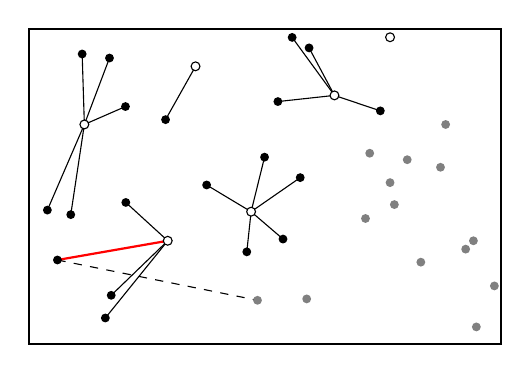
\begin{tikzpicture}[scale=0.4]
\draw [<->,thick] (0,0) rectangle (15,10) {};
\draw [-,dashed](0.909705882352941, 2.659076923076923) -- (7.261764705882353, 1.3796923076923076);
\fill [gray](7.261764705882353, 1.3796923076923076)circle(4pt);
\fill [gray](10.690588235294118, 3.9763076923076923)circle(4pt);
\draw [-](3.0697058823529413, 7.531076923076923) -- (1.7647058823529411, 6.961538461538462);
\fill(3.0697058823529413, 7.531076923076923)circle(4pt);
\draw [-](11.161764705882353, 7.393538461538461) -- (9.705882352941176, 7.884615384615385);
\fill(11.161764705882353, 7.393538461538461)circle(4pt);
\draw [-](2.4308823529411763, 0.8175384615384615) -- (4.411764705882353, 3.269230769230769);
\fill(2.4308823529411763, 0.8175384615384615)circle(4pt);
\fill [gray](11.60735294117647, 4.418461538461538)circle(4pt);
\draw [-](2.617058823529412, 1.5375384615384617) -- (4.411764705882353, 3.269230769230769);
\fill(2.617058823529412, 1.5375384615384617)circle(4pt);
\draw [-](8.617941176470588, 5.274153846153846) -- (7.0588235294117645, 4.1923076923076925);
\fill(8.617941176470588, 5.274153846153846)circle(4pt);
\draw [-](0.5902941176470589, 4.243076923076923) -- (1.7647058823529411, 6.961538461538462);
\fill(0.5902941176470589, 4.243076923076923)circle(4pt);
\draw [-](1.695, 9.199076923076923) -- (1.7647058823529411, 6.961538461538462);
\fill(1.695, 9.199076923076923)circle(4pt);
\draw [-](4.342941176470588, 7.114769230769231) -- (5.294117647058823, 8.807692307692308);
\fill(4.342941176470588, 7.114769230769231)circle(4pt);
\draw [-](8.899411764705881, 9.392923076923077) -- (9.705882352941176, 7.884615384615385);
\fill(8.899411764705881, 9.392923076923077)circle(4pt);
\draw [-](7.485882352941177, 5.924) -- (7.0588235294117645, 4.1923076923076925);
\fill(7.485882352941177, 5.924)circle(4pt);
\fill [gray](14.21029411764706, 0.5341538461538462)circle(4pt);
\fill [gray](14.78294117647059, 1.8356923076923077)circle(4pt);
\fill [gray](13.871470588235294, 3.0033846153846158)circle(4pt);
\draw [-](1.333235294117647, 4.099076923076923) -- (1.7647058823529411, 6.961538461538462);
\fill(1.333235294117647, 4.099076923076923)circle(4pt);
\draw [-](2.5623529411764707, 9.070769230769232) -- (1.7647058823529411, 6.961538461538462);
\fill(2.5623529411764707, 9.070769230769232)circle(4pt);
\fill [gray](12.015882352941176, 5.842769230769231)circle(4pt);
\fill [gray](12.448235294117648, 2.5898461538461537)circle(4pt);
\draw [-,thick,red](0.909705882352941, 2.659076923076923) -- (4.411764705882353, 3.269230769230769);
\fill(0.909705882352941, 2.659076923076923)circle(4pt);
\draw [-](3.0811764705882356, 4.485846153846154) -- (4.411764705882353, 3.269230769230769);
\fill(3.0811764705882356, 4.485846153846154)circle(4pt);
\draw [-](8.362058823529411, 9.726153846153846) -- (9.705882352941176, 7.884615384615385);
\fill(8.362058823529411, 9.726153846153846)circle(4pt);
\fill [gray](10.824705882352943, 6.048615384615385)circle(4pt);
\draw [-](5.647058823529412, 5.040615384615384) -- (7.0588235294117645, 4.1923076923076925);
\fill(5.647058823529412, 5.040615384615384)circle(4pt);
\draw [-](8.071764705882353, 3.3236923076923075) -- (7.0588235294117645, 4.1923076923076925);
\fill(8.071764705882353, 3.3236923076923075)circle(4pt);
\fill [gray](13.072058823529412, 5.602769230769231)circle(4pt);
\draw [-](6.922058823529412, 2.917538461538462) -- (7.0588235294117645, 4.1923076923076925);
\fill(6.922058823529412, 2.917538461538462)circle(4pt);
\draw [-](7.909411764705883, 7.688923076923077) -- (9.705882352941176, 7.884615384615385);
\fill(7.909411764705883, 7.688923076923077)circle(4pt);
\fill [gray](8.823529411764707, 1.4230769230769231)circle(4pt);
\fill [gray](11.470588235294118, 5.115384615384615)circle(4pt);
\fill [gray](13.235294117647058, 6.961538461538462)circle(4pt);
\fill [gray](14.117647058823529, 3.269230769230769)circle(4pt);
\fill [white](1.7647058823529411, 6.961538461538462)circle(4pt);
\draw [black](1.7647058823529411, 6.961538461538462)circle(4pt);
\fill [white](4.411764705882353, 3.269230769230769)circle(4pt);
\draw [black](4.411764705882353, 3.269230769230769)circle(4pt);
\fill [white](5.294117647058823, 8.807692307692308)circle(4pt);
\draw [black](5.294117647058823, 8.807692307692308)circle(4pt);
\fill [white](9.705882352941176, 7.884615384615385)circle(4pt);
\draw [black](9.705882352941176, 7.884615384615385)circle(4pt);
\fill [white](11.470588235294118, 9.73076923076923)circle(4pt);
\draw [black](11.470588235294118, 9.73076923076923)circle(4pt);
\fill [white](7.0588235294117645, 4.1923076923076925)circle(4pt);
\draw [black](7.0588235294117645, 4.1923076923076925)circle(4pt);
\end{tikzpicture}
\caption[Illustration of the lower bound calculation.]{Illustration of the lower bound calculation. The dashed line represents the value for the lower bound. Since the value is larger than the current objective function, in red, if there has been found a branch with a better solution, then the current branch is pruned.}
\label{fig:bound}
\end{figure}



\section{Delaunay Assisted Branch-and-Bound}
\label{alg:da}

Most of the operations in the branch-and-bound approach described in Section \ref{alg:bb} have at least linear time complexity for both the best and expected cases. We can speed these up by implementing incrementally built Delaunay triangulations, which can be used to accelerate point location queries. To aid the calculations, the points are pre-processed and sorted by a Hilbert Curve approximation of a sufficiently high order.

\paragraph{Inserting a Centroid}
In order to take advantage of Delaunay triangulations, each time a centroid is chosen, it must be included in the Delaunay triangulation. This means that the triangulation must be updated. Inserting a point in a triangulation with $K$ vertices using the Bowyer-Watson algorithm described in Section \ref{sect:dtconst} takes an estimated $\mathcal{O}(\log{K})$ for a uniformly distributed set of points \cite{tricomplex}.
After a centroid $c$ is included in a Delaunay triangulation, it is possible to know which other centroids are its Voronoi neighbours. This is due to the duality between Delaunay triangulations and Voronoi diagrams.
Since Voronoi diagrams partition the space into regions by distance to the centroids, we only need to check the subset of non-centroids assigned to the direct neighbours of $c$ to find which points should change assignment to $c$. 
This property lowers the expected number of comparisons to make. Since the average number of Voronoi neighbours per centroid in any given diagram cannot exceed six \cite{tricard2,tricard1}, the number of points to be compared in a uniformly distributed set of non-centroids should not include all non-centroids, but only a small fraction of them.
Despite the lower number of comparisons, the worst-case time complexity still takes $\mathcal{O}(N)$ time to complete, and in the worst case scenario it can still require a check through all non-centroids, which can all be neighbours of $c$.
If the objective function maximiser is assigned to $c$, all non-centroids can be candidates to become the new maximiser, so a linear search through all the non-centroids must be done, to see which one is now the farthest away from its centroid. Figure \ref{fig:gncent} illustrates this operation.

\begin{figure}[!h]
\centering
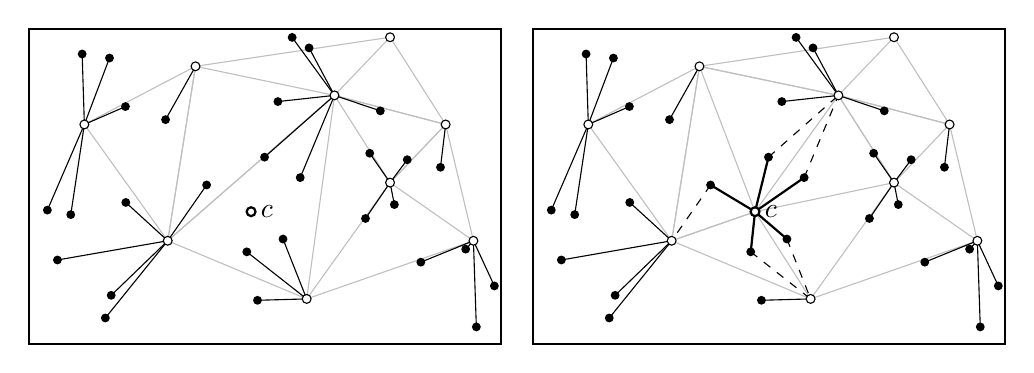
\begin{tikzpicture}[scale=0.4]

\draw [<->,thick] (0,0) rectangle (15,10) {};

\draw [-,gray!50] (11.471,5.115) -- (8.824,1.423);
\draw [-,gray!50] (13.235,6.962) -- (11.471,5.115);
\draw [-,gray!50] (13.235,6.962) -- (11.471,9.731);
\draw [-,gray!50] (9.706,7.885) -- (4.412,3.269);
\draw [-,gray!50] (11.471,5.115) -- (14.118,3.269);
\draw [-,gray!50] (5.294,8.808) -- (1.765,6.962);
\draw [-,gray!50] (11.471,5.115) -- (13.235,6.962);
\draw [-,gray!50] (5.294,8.808) -- (4.412,3.269);
\draw [-,gray!50] (8.824,1.423) -- (14.118,3.269);
\draw [-,gray!50] (5.294,8.808) -- (11.471,9.731);
\draw [-,gray!50] (13.235,6.962) -- (9.706,7.885);
\draw [-,gray!50] (4.412,3.269) -- (8.824,1.423);
\draw [-,gray!50] (4.412,3.269) -- (1.765,6.962);
\draw [-,gray!50] (4.412,3.269) -- (5.294,8.808);
\draw [-,gray!50] (9.706,7.885) -- (11.471,9.731);
\draw [-,gray!50] (9.706,7.885) -- (8.824,1.423);
\draw [-,gray!50] (4.412,3.269) -- (9.706,7.885);
\draw [-,gray!50] (11.471,5.115) -- (9.706,7.885);
\draw [-,gray!50] (9.706,7.885) -- (13.235,6.962);
\draw [-,gray!50] (13.235,6.962) -- (14.118,3.269);
\draw [-,gray!50] (5.294,8.808) -- (9.706,7.885);
\draw [-](7.261764705882353, 1.3796923076923076) -- (8.823529411764707, 1.4230769230769231);
\draw [-](10.690588235294118, 3.9763076923076923) -- (11.470588235294118, 5.115384615384615);
\draw [-](3.0697058823529413, 7.531076923076923) -- (1.7647058823529411, 6.961538461538462);
\draw [-](11.161764705882353, 7.393538461538461) -- (9.705882352941176, 7.884615384615385);
\draw [-](2.4308823529411763, 0.8175384615384615) -- (4.411764705882353, 3.269230769230769);
\draw [-](11.60735294117647, 4.418461538461538) -- (11.470588235294118, 5.115384615384615);
\draw [-](2.617058823529412, 1.5375384615384617) -- (4.411764705882353, 3.269230769230769);
\draw [-](8.617941176470588, 5.274153846153846) -- (9.705882352941176, 7.884615384615385);
\draw [-](0.5902941176470589, 4.243076923076923) -- (1.7647058823529411, 6.961538461538462);
\draw [-](1.695, 9.199076923076923) -- (1.7647058823529411, 6.961538461538462);
\draw [-](4.342941176470588, 7.114769230769231) -- (5.294117647058823, 8.807692307692308);
\draw [-](8.899411764705881, 9.392923076923077) -- (9.705882352941176, 7.884615384615385);
\draw [-](7.485882352941177, 5.924) -- (9.705882352941176, 7.884615384615385);
\draw [-](14.21029411764706, 0.5341538461538462) -- (14.117647058823529, 3.269230769230769);
\draw [-](14.78294117647059, 1.8356923076923077) -- (14.117647058823529, 3.269230769230769);
\draw [-](13.871470588235294, 3.0033846153846158) -- (14.117647058823529, 3.269230769230769);
\draw [-](1.333235294117647, 4.099076923076923) -- (1.7647058823529411, 6.961538461538462);
\draw [-](2.5623529411764707, 9.070769230769232) -- (1.7647058823529411, 6.961538461538462);
\draw [-](12.015882352941176, 5.842769230769231) -- (11.470588235294118, 5.115384615384615);
\draw [-](12.448235294117648, 2.5898461538461537) -- (14.117647058823529, 3.269230769230769);
\draw [-](0.909705882352941, 2.659076923076923) -- (4.411764705882353, 3.269230769230769);
\draw [-](3.0811764705882356, 4.485846153846154) -- (4.411764705882353, 3.269230769230769);
\draw [-](8.362058823529411, 9.726153846153846) -- (9.705882352941176, 7.884615384615385);
\draw [-](10.824705882352943, 6.048615384615385) -- (11.470588235294118, 5.115384615384615);
\draw [-](5.647058823529412, 5.040615384615384) -- (4.411764705882353, 3.269230769230769);
\draw [-](8.071764705882353, 3.3236923076923075) -- (8.823529411764707, 1.4230769230769231);
\draw [-](13.072058823529412, 5.602769230769231) -- (13.235294117647058, 6.961538461538462);
\draw [-](6.922058823529412, 2.917538461538462) -- (8.823529411764707, 1.4230769230769231);
\draw [-](7.909411764705883, 7.688923076923077) -- (9.705882352941176, 7.884615384615385);
\fill [white](1.7647058823529411, 6.961538461538462)circle(4pt);
\draw (1.7647058823529411, 6.961538461538462)circle(4pt);
\fill [white](4.411764705882353, 3.269230769230769)circle(4pt);
\draw (4.411764705882353, 3.269230769230769)circle(4pt);
\fill [white](5.294117647058823, 8.807692307692308)circle(4pt);
\draw (5.294117647058823, 8.807692307692308)circle(4pt);
\fill [white](8.823529411764707, 1.4230769230769231)circle(4pt);
\draw (8.823529411764707, 1.4230769230769231)circle(4pt);
\fill [white](9.705882352941176, 7.884615384615385)circle(4pt);
\draw (9.705882352941176, 7.884615384615385)circle(4pt);
\fill [white](11.470588235294118, 5.115384615384615)circle(4pt);
\draw (11.470588235294118, 5.115384615384615)circle(4pt);
\fill [white](11.470588235294118, 9.73076923076923)circle(4pt);
\draw (11.470588235294118, 9.73076923076923)circle(4pt);
\fill [white](13.235294117647058, 6.961538461538462)circle(4pt);
\draw (13.235294117647058, 6.961538461538462)circle(4pt);
\fill [white](14.117647058823529, 3.269230769230769)circle(4pt);
\draw (14.117647058823529, 3.269230769230769)circle(4pt);
\fill [white](7.0588235294117645, 4.1923076923076925)circle(4pt);
\draw [thick](7.0588235294117645, 4.1923076923076925)circle(4pt);
\fill(7.261764705882353, 1.3796923076923076)circle(4pt);
\fill(10.690588235294118, 3.9763076923076923)circle(4pt);
\fill(3.0697058823529413, 7.531076923076923)circle(4pt);
\fill(11.161764705882353, 7.393538461538461)circle(4pt);
\fill(2.4308823529411763, 0.8175384615384615)circle(4pt);
\fill(11.60735294117647, 4.418461538461538)circle(4pt);
\fill(2.617058823529412, 1.5375384615384617)circle(4pt);
\fill(8.617941176470588, 5.274153846153846)circle(4pt);
\fill(0.5902941176470589, 4.243076923076923)circle(4pt);
\fill(1.695, 9.199076923076923)circle(4pt);
\fill(4.342941176470588, 7.114769230769231)circle(4pt);
\fill(8.899411764705881, 9.392923076923077)circle(4pt);
\fill(7.485882352941177, 5.924)circle(4pt);
\fill(14.21029411764706, 0.5341538461538462)circle(4pt);
\fill(14.78294117647059, 1.8356923076923077)circle(4pt);
\fill(13.871470588235294, 3.0033846153846158)circle(4pt);
\fill(1.333235294117647, 4.099076923076923)circle(4pt);
\fill(2.5623529411764707, 9.070769230769232)circle(4pt);
\fill(12.015882352941176, 5.842769230769231)circle(4pt);
\fill(12.448235294117648, 2.5898461538461537)circle(4pt);
\fill(0.909705882352941, 2.659076923076923)circle(4pt);
\fill(3.0811764705882356, 4.485846153846154)circle(4pt);
\fill(8.362058823529411, 9.726153846153846)circle(4pt);
\fill(10.824705882352943, 6.048615384615385)circle(4pt);
\fill(5.647058823529412, 5.040615384615384)circle(4pt);
\fill(8.071764705882353, 3.3236923076923075)circle(4pt);
\fill(13.072058823529412, 5.602769230769231)circle(4pt);
\fill(6.922058823529412, 2.917538461538462)circle(4pt);
\fill(7.909411764705883, 7.688923076923077)circle(4pt);
\node at (7.0588235294117645, 4.1923076923076925)[right] {$c$};
\begin{scope}[shift={(16,0)}]
\draw [<->,thick] (0,0) rectangle (15,10) {};
\draw [-,gray!50] (11.471,5.115) -- (8.824,1.423);
\draw [-,gray!50] (9.706,7.885) -- (5.294,8.808);
\draw [-,gray!50] (11.471,5.115) -- (7.059,4.192);
\draw [-,gray!50] (13.235,6.962) -- (11.471,5.115);
\draw [-,gray!50] (7.059,4.192) -- (4.412,3.269);
\draw [-,gray!50] (4.412,3.269) -- (7.059,4.192);
\draw [-,gray!50] (11.471,5.115) -- (14.118,3.269);
\draw [-,gray!50] (13.235,6.962) -- (11.471,9.731);
\draw [-,gray!50] (5.294,8.808) -- (1.765,6.962);
\draw [-,gray!50] (13.235,6.962) -- (14.118,3.269);
\draw [-,gray!50] (5.294,8.808) -- (7.059,4.192);
\draw [-,gray!50] (5.294,8.808) -- (4.412,3.269);
\draw [-,gray!50] (8.824,1.423) -- (14.118,3.269);
\draw [-,gray!50] (5.294,8.808) -- (11.471,9.731);
\draw [-,gray!50] (13.235,6.962) -- (9.706,7.885);
\draw [-,gray!50] (9.706,7.885) -- (11.471,5.115);
\draw [-,gray!50] (4.412,3.269) -- (8.824,1.423);
\draw [-,gray!50] (4.412,3.269) -- (1.765,6.962);
\draw [-,gray!50] (4.412,3.269) -- (5.294,8.808);
\draw [-,gray!50] (9.706,7.885) -- (11.471,9.731);
\draw [-,gray!50] (9.706,7.885) -- (7.059,4.192);
\draw [-,gray!50] (11.471,5.115) -- (9.706,7.885);
\draw [-,gray!50] (9.706,7.885) -- (13.235,6.962);
\draw [-,gray!50] (7.059,4.192) -- (8.824,1.423);
\draw [-,gray!50] (5.294,8.808) -- (9.706,7.885);
\draw [-](7.261764705882353, 1.3796923076923076) -- (8.823529411764707, 1.4230769230769231);
\draw [-](10.690588235294118, 3.9763076923076923) -- (11.470588235294118, 5.115384615384615);
\draw [-](3.0697058823529413, 7.531076923076923) -- (1.7647058823529411, 6.961538461538462);
\draw [-](11.161764705882353, 7.393538461538461) -- (9.705882352941176, 7.884615384615385);
\draw [-](2.4308823529411763, 0.8175384615384615) -- (4.411764705882353, 3.269230769230769);
\draw [-](11.60735294117647, 4.418461538461538) -- (11.470588235294118, 5.115384615384615);
\draw [-](2.617058823529412, 1.5375384615384617) -- (4.411764705882353, 3.269230769230769);
\draw [-,dashed](8.617941176470588, 5.274153846153846) -- (9.705882352941176, 7.884615384615385);
\draw [-](0.5902941176470589, 4.243076923076923) -- (1.7647058823529411, 6.961538461538462);
\draw [-](1.695, 9.199076923076923) -- (1.7647058823529411, 6.961538461538462);
\draw [-](4.342941176470588, 7.114769230769231) -- (5.294117647058823, 8.807692307692308);
\draw [-](8.899411764705881, 9.392923076923077) -- (9.705882352941176, 7.884615384615385);
\draw [-,dashed](7.485882352941177, 5.924) -- (9.705882352941176, 7.884615384615385);
\draw [-](14.21029411764706, 0.5341538461538462) -- (14.117647058823529, 3.269230769230769);
\draw [-](14.78294117647059, 1.8356923076923077) -- (14.117647058823529, 3.269230769230769);
\draw [-](13.871470588235294, 3.0033846153846158) -- (14.117647058823529, 3.269230769230769);
\draw [-](1.333235294117647, 4.099076923076923) -- (1.7647058823529411, 6.961538461538462);
\draw [-](2.5623529411764707, 9.070769230769232) -- (1.7647058823529411, 6.961538461538462);
\draw [-](12.015882352941176, 5.842769230769231) -- (11.470588235294118, 5.115384615384615);
\draw [-](12.448235294117648, 2.5898461538461537) -- (14.117647058823529, 3.269230769230769);
\draw [-](0.909705882352941, 2.659076923076923) -- (4.411764705882353, 3.269230769230769);
\draw [-](3.0811764705882356, 4.485846153846154) -- (4.411764705882353, 3.269230769230769);
\draw [-](8.362058823529411, 9.726153846153846) -- (9.705882352941176, 7.884615384615385);
\draw [-](10.824705882352943, 6.048615384615385) -- (11.470588235294118, 5.115384615384615);
\draw [-,dashed](5.647058823529412, 5.040615384615384) -- (4.411764705882353, 3.269230769230769);
\draw [-,dashed](8.071764705882353, 3.3236923076923075) -- (8.823529411764707, 1.4230769230769231);
\draw [-](13.072058823529412, 5.602769230769231) -- (13.235294117647058, 6.961538461538462);
\draw [-,dashed](6.922058823529412, 2.917538461538462) -- (8.823529411764707, 1.4230769230769231);
\draw [-](7.909411764705883, 7.688923076923077) -- (9.705882352941176, 7.884615384615385);
\draw [-,thick](8.617941176470588, 5.274153846153846) -- (7.0588235294117645, 4.1923076923076925);
\draw [-,thick](7.485882352941177, 5.924) -- (7.0588235294117645, 4.1923076923076925);
\draw [-,thick](5.647058823529412, 5.040615384615384) -- (7.0588235294117645, 4.1923076923076925);
\draw [-,thick](8.071764705882353, 3.3236923076923075) -- (7.0588235294117645, 4.1923076923076925);
\draw [-,thick](6.922058823529412, 2.917538461538462) -- (7.0588235294117645, 4.1923076923076925);
\fill [white](1.7647058823529411, 6.961538461538462)circle(4pt);
\draw (1.7647058823529411, 6.961538461538462)circle(4pt);
\fill [white](4.411764705882353, 3.269230769230769)circle(4pt);
\draw (4.411764705882353, 3.269230769230769)circle(4pt);
\fill [white](5.294117647058823, 8.807692307692308)circle(4pt);
\draw (5.294117647058823, 8.807692307692308)circle(4pt);
\fill [white](8.823529411764707, 1.4230769230769231)circle(4pt);
\draw (8.823529411764707, 1.4230769230769231)circle(4pt);
\fill [white](9.705882352941176, 7.884615384615385)circle(4pt);
\draw (9.705882352941176, 7.884615384615385)circle(4pt);
\fill [white](11.470588235294118, 5.115384615384615)circle(4pt);
\draw (11.470588235294118, 5.115384615384615)circle(4pt);
\fill [white](11.470588235294118, 9.73076923076923)circle(4pt);
\draw (11.470588235294118, 9.73076923076923)circle(4pt);
\fill [white](13.235294117647058, 6.961538461538462)circle(4pt);
\draw (13.235294117647058, 6.961538461538462)circle(4pt);
\fill [white](14.117647058823529, 3.269230769230769)circle(4pt);
\draw (14.117647058823529, 3.269230769230769)circle(4pt);
\fill [white](7.0588235294117645, 4.1923076923076925)circle(4pt);
\draw [thick](7.0588235294117645, 4.1923076923076925)circle(4pt);
\fill(7.261764705882353, 1.3796923076923076)circle(4pt);
\fill(10.690588235294118, 3.9763076923076923)circle(4pt);
\fill(3.0697058823529413, 7.531076923076923)circle(4pt);
\fill(11.161764705882353, 7.393538461538461)circle(4pt);
\fill(2.4308823529411763, 0.8175384615384615)circle(4pt);
\fill(11.60735294117647, 4.418461538461538)circle(4pt);
\fill(2.617058823529412, 1.5375384615384617)circle(4pt);
\fill(8.617941176470588, 5.274153846153846)circle(4pt);
\fill(0.5902941176470589, 4.243076923076923)circle(4pt);
\fill(1.695, 9.199076923076923)circle(4pt);
\fill(4.342941176470588, 7.114769230769231)circle(4pt);
\fill(8.899411764705881, 9.392923076923077)circle(4pt);
\fill(7.485882352941177, 5.924)circle(4pt);
\fill(14.21029411764706, 0.5341538461538462)circle(4pt);
\fill(14.78294117647059, 1.8356923076923077)circle(4pt);
\fill(13.871470588235294, 3.0033846153846158)circle(4pt);
\fill(1.333235294117647, 4.099076923076923)circle(4pt);
\fill(2.5623529411764707, 9.070769230769232)circle(4pt);
\fill(12.015882352941176, 5.842769230769231)circle(4pt);
\fill(12.448235294117648, 2.5898461538461537)circle(4pt);
\fill(0.909705882352941, 2.659076923076923)circle(4pt);
\fill(3.0811764705882356, 4.485846153846154)circle(4pt);
\fill(8.362058823529411, 9.726153846153846)circle(4pt);
\fill(10.824705882352943, 6.048615384615385)circle(4pt);
\fill(5.647058823529412, 5.040615384615384)circle(4pt);
\fill(8.071764705882353, 3.3236923076923075)circle(4pt);
\fill(13.072058823529412, 5.602769230769231)circle(4pt);
\fill(6.922058823529412, 2.917538461538462)circle(4pt);
\fill(7.909411764705883, 7.688923076923077)circle(4pt);
\node at (7.0588235294117645, 4.1923076923076925)[right] {$c$};
\end{scope}
\end{tikzpicture}
\caption[Illustration of a centroid insertion using the geometric method]{Illustration of a centroid insertion $c$ using the geometric method. The Delaunay triangulation is updated and only the neighbours of $c$ need to be checked for assignment updates.}
\label{fig:gncent}
\end{figure}


\paragraph{Inserting a Non-Centroid}
Since there is a triangulation built, using the centroids as its vertices, finding the closest centroid $c$ to a new non-centroid $n$ is simply a matter of using the greedy routing algorithm to find $c$ \cite{greedyroute}.
The greedy routing algorithm has a worst-case time complexity of $\mathcal{O}(K)$. This happens when the search starts from the farthest centroid from $n$, and all centroids are either in the direction of $n$, or are neighbours of the centroids that are. 
The last centroid returned by the greedy routing algorithm can be used to start the new query. Since the points are inserted ordered by a Hilbert curve approximation, each consecutive point should minimise the position variation from the last.
This means that, ideally, each inserted non-centroid $n$ is close to its respective optimally positioned centroid $c$, and it only needs to calculate the distances to the neighbours of $c$ in order to guarantee that $c$ is indeed the correct centroid.
The aforementioned property of the average six neighbours for each centroid means that the expected time for a query starting at the right centroid would be $\mathcal{O}(1)$. This represents the best case scenario, and is heuristically approximated by the Hilbert curves. The time complexity of inserting one non-centroid is still $\mathcal{O}(K)$ for the worst case. 
However, the insertion of a large number of uniformly distributed points \emph{should} behave closer to $\mathcal{O}(\sqrt{K})$ time per point. If a rectangular area has $N$ points, the longest path would be a diagonal. The diagonal, like the sides, has close to $\sqrt{N}$ number of points, in an area with a sufficiently good uniformity of points in it. Figure \ref{fig:gnncent} illustrates this operation.

\begin{figure}[H]
\centering
\begin{minipage}{0.45\linewidth}
\centering
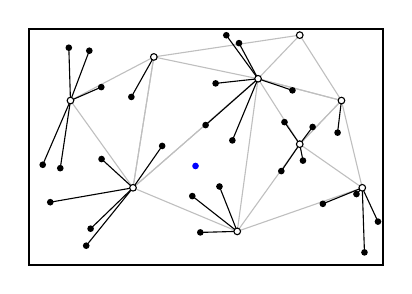
\begin{tikzpicture}[scale=0.3]

\draw [<->,thick] (0,0) rectangle (15,10) {};
\draw [-,gray!50] (11.471,5.115) -- (8.824,1.423);
\draw [-,gray!50] (13.235,6.962) -- (11.471,5.115);
\draw [-,gray!50] (13.235,6.962) -- (11.471,9.731);
\draw [-,gray!50] (9.706,7.885) -- (4.412,3.269);
\draw [-,gray!50] (11.471,5.115) -- (14.118,3.269);
\draw [-,gray!50] (5.294,8.808) -- (1.765,6.962);
\draw [-,gray!50] (11.471,5.115) -- (13.235,6.962);
\draw [-,gray!50] (5.294,8.808) -- (4.412,3.269);
\draw [-,gray!50] (8.824,1.423) -- (14.118,3.269);
\draw [-,gray!50] (5.294,8.808) -- (11.471,9.731);
\draw [-,gray!50] (13.235,6.962) -- (9.706,7.885);
\draw [-,gray!50] (4.412,3.269) -- (8.824,1.423);
\draw [-,gray!50] (4.412,3.269) -- (1.765,6.962);
\draw [-,gray!50] (4.412,3.269) -- (5.294,8.808);
\draw [-,gray!50] (9.706,7.885) -- (11.471,9.731);
\draw [-,gray!50] (9.706,7.885) -- (8.824,1.423);
\draw [-,gray!50] (4.412,3.269) -- (9.706,7.885);
\draw [-,gray!50] (11.471,5.115) -- (9.706,7.885);
\draw [-,gray!50] (9.706,7.885) -- (13.235,6.962);
\draw [-,gray!50] (13.235,6.962) -- (14.118,3.269);
\draw [-,gray!50] (5.294,8.808) -- (9.706,7.885);
\draw [-](7.261764705882353, 1.3796923076923076) -- (8.823529411764707, 1.4230769230769231);
\draw [-](10.690588235294118, 3.9763076923076923) -- (11.470588235294118, 5.115384615384615);
\draw [-](3.0697058823529413, 7.531076923076923) -- (1.7647058823529411, 6.961538461538462);
\draw [-](11.161764705882353, 7.393538461538461) -- (9.705882352941176, 7.884615384615385);
\draw [-](2.4308823529411763, 0.8175384615384615) -- (4.411764705882353, 3.269230769230769);
\draw [-](11.60735294117647, 4.418461538461538) -- (11.470588235294118, 5.115384615384615);
\draw [-](2.617058823529412, 1.5375384615384617) -- (4.411764705882353, 3.269230769230769);
\draw [-](8.617941176470588, 5.274153846153846) -- (9.705882352941176, 7.884615384615385);
\draw [-](0.5902941176470589, 4.243076923076923) -- (1.7647058823529411, 6.961538461538462);
\draw [-](1.695, 9.199076923076923) -- (1.7647058823529411, 6.961538461538462);
\draw [-](4.342941176470588, 7.114769230769231) -- (5.294117647058823, 8.807692307692308);
\draw [-](8.899411764705881, 9.392923076923077) -- (9.705882352941176, 7.884615384615385);
\draw [-](7.485882352941177, 5.924) -- (9.705882352941176, 7.884615384615385);
\draw [-](14.21029411764706, 0.5341538461538462) -- (14.117647058823529, 3.269230769230769);
\draw [-](14.78294117647059, 1.8356923076923077) -- (14.117647058823529, 3.269230769230769);
\draw [-](13.871470588235294, 3.0033846153846158) -- (14.117647058823529, 3.269230769230769);
\draw [-](1.333235294117647, 4.099076923076923) -- (1.7647058823529411, 6.961538461538462);
\draw [-](2.5623529411764707, 9.070769230769232) -- (1.7647058823529411, 6.961538461538462);
\draw [-](12.015882352941176, 5.842769230769231) -- (11.470588235294118, 5.115384615384615);
\draw [-](12.448235294117648, 2.5898461538461537) -- (14.117647058823529, 3.269230769230769);
\draw [-](0.909705882352941, 2.659076923076923) -- (4.411764705882353, 3.269230769230769);
\draw [-](3.0811764705882356, 4.485846153846154) -- (4.411764705882353, 3.269230769230769);
\draw [-](8.362058823529411, 9.726153846153846) -- (9.705882352941176, 7.884615384615385);
\draw [-](10.824705882352943, 6.048615384615385) -- (11.470588235294118, 5.115384615384615);
\draw [-](5.647058823529412, 5.040615384615384) -- (4.411764705882353, 3.269230769230769);
\draw [-](8.071764705882353, 3.3236923076923075) -- (8.823529411764707, 1.4230769230769231);
\draw [-](13.072058823529412, 5.602769230769231) -- (13.235294117647058, 6.961538461538462);
\draw [-](6.922058823529412, 2.917538461538462) -- (8.823529411764707, 1.4230769230769231);
\draw [-](7.909411764705883, 7.688923076923077) -- (9.705882352941176, 7.884615384615385);
\fill [white](1.7647058823529411, 6.961538461538462)circle(4pt);
\draw (1.7647058823529411, 6.961538461538462)circle(4pt);
\fill [white](4.411764705882353, 3.269230769230769)circle(4pt);
\draw (4.411764705882353, 3.269230769230769)circle(4pt);
\fill [white](5.294117647058823, 8.807692307692308)circle(4pt);
\draw (5.294117647058823, 8.807692307692308)circle(4pt);
\fill [white](8.823529411764707, 1.4230769230769231)circle(4pt);
\draw (8.823529411764707, 1.4230769230769231)circle(4pt);
\fill [white](9.705882352941176, 7.884615384615385)circle(4pt);
\draw (9.705882352941176, 7.884615384615385)circle(4pt);
\fill [white](11.470588235294118, 5.115384615384615)circle(4pt);
\draw (11.470588235294118, 5.115384615384615)circle(4pt);
\fill [white](11.470588235294118, 9.73076923076923)circle(4pt);
\draw (11.470588235294118, 9.73076923076923)circle(4pt);
\fill [white](13.235294117647058, 6.961538461538462)circle(4pt);
\draw (13.235294117647058, 6.961538461538462)circle(4pt);
\fill [white](14.117647058823529, 3.269230769230769)circle(4pt);
\draw (14.117647058823529, 3.269230769230769)circle(4pt);
\fill [blue](7.0588235294117645, 4.1923076923076925)circle(4pt);
\fill(7.261764705882353, 1.3796923076923076)circle(4pt);
\fill(10.690588235294118, 3.9763076923076923)circle(4pt);
\fill(3.0697058823529413, 7.531076923076923)circle(4pt);
\fill(11.161764705882353, 7.393538461538461)circle(4pt);
\fill(2.4308823529411763, 0.8175384615384615)circle(4pt);
\fill(11.60735294117647, 4.418461538461538)circle(4pt);
\fill(2.617058823529412, 1.5375384615384617)circle(4pt);
\fill(8.617941176470588, 5.274153846153846)circle(4pt);
\fill(0.5902941176470589, 4.243076923076923)circle(4pt);
\fill(1.695, 9.199076923076923)circle(4pt);
\fill(4.342941176470588, 7.114769230769231)circle(4pt);
\fill(8.899411764705881, 9.392923076923077)circle(4pt);
\fill(7.485882352941177, 5.924)circle(4pt);
\fill(14.21029411764706, 0.5341538461538462)circle(4pt);
\fill(14.78294117647059, 1.8356923076923077)circle(4pt);
\fill(13.871470588235294, 3.0033846153846158)circle(4pt);
\fill(1.333235294117647, 4.099076923076923)circle(4pt);
\fill(2.5623529411764707, 9.070769230769232)circle(4pt);
\fill(12.015882352941176, 5.842769230769231)circle(4pt);
\fill(12.448235294117648, 2.5898461538461537)circle(4pt);
\fill(0.909705882352941, 2.659076923076923)circle(4pt);
\fill(3.0811764705882356, 4.485846153846154)circle(4pt);
\fill(8.362058823529411, 9.726153846153846)circle(4pt);
\fill(10.824705882352943, 6.048615384615385)circle(4pt);
\fill(5.647058823529412, 5.040615384615384)circle(4pt);
\fill(8.071764705882353, 3.3236923076923075)circle(4pt);
\fill(13.072058823529412, 5.602769230769231)circle(4pt);
\fill(6.922058823529412, 2.917538461538462)circle(4pt);
\fill(7.909411764705883, 7.688923076923077)circle(4pt);
\end{tikzpicture}\end{minipage}\begin{minipage}{0.45\linewidth}\centering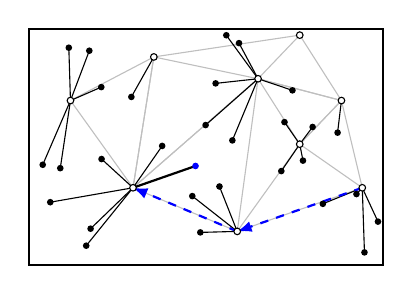
\begin{tikzpicture}[scale=0.3]
\draw [<->,thick] (0,0) rectangle (15,10) {};
\draw [-,gray!50] (11.471,5.115) -- (8.824,1.423);
\draw [-,gray!50] (13.235,6.962) -- (11.471,5.115);
\draw [-,gray!50] (13.235,6.962) -- (11.471,9.731);
\draw [-,gray!50] (9.706,7.885) -- (4.412,3.269);
\draw [-,gray!50] (11.471,5.115) -- (14.118,3.269);
\draw [-,gray!50] (5.294,8.808) -- (1.765,6.962);
\draw [-,gray!50] (11.471,5.115) -- (13.235,6.962);
\draw [-,gray!50] (5.294,8.808) -- (4.412,3.269);
\draw [-,gray!50] (8.824,1.423) -- (14.118,3.269);
\draw [-,gray!50] (5.294,8.808) -- (11.471,9.731);
\draw [-,gray!50] (13.235,6.962) -- (9.706,7.885);
\draw [-,gray!50] (4.412,3.269) -- (8.824,1.423);
\draw [-,gray!50] (4.412,3.269) -- (1.765,6.962);
\draw [-,gray!50] (4.412,3.269) -- (5.294,8.808);
\draw [-,gray!50] (9.706,7.885) -- (11.471,9.731);
\draw [-,gray!50] (9.706,7.885) -- (8.824,1.423);
\draw [-,gray!50] (4.412,3.269) -- (9.706,7.885);
\draw [-,gray!50] (11.471,5.115) -- (9.706,7.885);
\draw [-,gray!50] (9.706,7.885) -- (13.235,6.962);
\draw [-,gray!50] (13.235,6.962) -- (14.118,3.269);
\draw [-,gray!50] (5.294,8.808) -- (9.706,7.885);
\draw [-](7.261764705882353, 1.3796923076923076) -- (8.823529411764707, 1.4230769230769231);
\draw [-](10.690588235294118, 3.9763076923076923) -- (11.470588235294118, 5.115384615384615);
\draw [-](3.0697058823529413, 7.531076923076923) -- (1.7647058823529411, 6.961538461538462);
\draw [-](11.161764705882353, 7.393538461538461) -- (9.705882352941176, 7.884615384615385);
\draw [-](2.4308823529411763, 0.8175384615384615) -- (4.411764705882353, 3.269230769230769);
\draw [-](11.60735294117647, 4.418461538461538) -- (11.470588235294118, 5.115384615384615);
\draw [-](2.617058823529412, 1.5375384615384617) -- (4.411764705882353, 3.269230769230769);
\draw [-](8.617941176470588, 5.274153846153846) -- (9.705882352941176, 7.884615384615385);
\draw [-](0.5902941176470589, 4.243076923076923) -- (1.7647058823529411, 6.961538461538462);
\draw [-](1.695, 9.199076923076923) -- (1.7647058823529411, 6.961538461538462);
\draw [-](4.342941176470588, 7.114769230769231) -- (5.294117647058823, 8.807692307692308);
\draw [-](8.899411764705881, 9.392923076923077) -- (9.705882352941176, 7.884615384615385);
\draw [-](7.485882352941177, 5.924) -- (9.705882352941176, 7.884615384615385);
\draw [-](14.21029411764706, 0.5341538461538462) -- (14.117647058823529, 3.269230769230769);
\draw [-](14.78294117647059, 1.8356923076923077) -- (14.117647058823529, 3.269230769230769);
\draw [-](13.871470588235294, 3.0033846153846158) -- (14.117647058823529, 3.269230769230769);
\draw [-](1.333235294117647, 4.099076923076923) -- (1.7647058823529411, 6.961538461538462);
\draw [-](2.5623529411764707, 9.070769230769232) -- (1.7647058823529411, 6.961538461538462);
\draw [-](12.015882352941176, 5.842769230769231) -- (11.470588235294118, 5.115384615384615);
\draw [-](12.448235294117648, 2.5898461538461537) -- (14.117647058823529, 3.269230769230769);
\draw [-](0.909705882352941, 2.659076923076923) -- (4.411764705882353, 3.269230769230769);
\draw [-](3.0811764705882356, 4.485846153846154) -- (4.411764705882353, 3.269230769230769);
\draw [-](8.362058823529411, 9.726153846153846) -- (9.705882352941176, 7.884615384615385);
\draw [-](10.824705882352943, 6.048615384615385) -- (11.470588235294118, 5.115384615384615);
\draw [-](5.647058823529412, 5.040615384615384) -- (4.411764705882353, 3.269230769230769);
\draw [-](8.071764705882353, 3.3236923076923075) -- (8.823529411764707, 1.4230769230769231);
\draw [-](13.072058823529412, 5.602769230769231) -- (13.235294117647058, 6.961538461538462);
\draw [-](6.922058823529412, 2.917538461538462) -- (8.823529411764707, 1.4230769230769231);
\draw [-](7.909411764705883, 7.688923076923077) -- (9.705882352941176, 7.884615384615385);
\draw [-,thick](7.0588235294117645, 4.1923076923076925) -- (4.411764705882353, 3.269230769230769);
\draw [->,>=latex,dashed,blue,thick](14.117647058823529, 3.269230769230769) -- (8.823529411764707, 1.4230769230769231);
\draw [->,>=latex,dashed,blue,thick](8.823529411764707, 1.4230769230769231) -- (4.411764705882353, 3.269230769230769);
\fill [white](1.7647058823529411, 6.961538461538462)circle(4pt);
\draw (1.7647058823529411, 6.961538461538462)circle(4pt);
\fill [white](4.411764705882353, 3.269230769230769)circle(4pt);
\draw (4.411764705882353, 3.269230769230769)circle(4pt);
\fill [white](5.294117647058823, 8.807692307692308)circle(4pt);
\draw (5.294117647058823, 8.807692307692308)circle(4pt);
\fill [white](8.823529411764707, 1.4230769230769231)circle(4pt);
\draw (8.823529411764707, 1.4230769230769231)circle(4pt);
\fill [white](9.705882352941176, 7.884615384615385)circle(4pt);
\draw (9.705882352941176, 7.884615384615385)circle(4pt);
\fill [white](11.470588235294118, 5.115384615384615)circle(4pt);
\draw (11.470588235294118, 5.115384615384615)circle(4pt);
\fill [white](11.470588235294118, 9.73076923076923)circle(4pt);
\draw (11.470588235294118, 9.73076923076923)circle(4pt);
\fill [white](13.235294117647058, 6.961538461538462)circle(4pt);
\draw (13.235294117647058, 6.961538461538462)circle(4pt);
\fill [white](14.117647058823529, 3.269230769230769)circle(4pt);
\draw (14.117647058823529, 3.269230769230769)circle(4pt);
\fill [blue](7.0588235294117645, 4.1923076923076925)circle(4pt);
\fill(7.261764705882353, 1.3796923076923076)circle(4pt);
\fill(10.690588235294118, 3.9763076923076923)circle(4pt);
\fill(3.0697058823529413, 7.531076923076923)circle(4pt);
\fill(11.161764705882353, 7.393538461538461)circle(4pt);
\fill(2.4308823529411763, 0.8175384615384615)circle(4pt);
\fill(11.60735294117647, 4.418461538461538)circle(4pt);
\fill(2.617058823529412, 1.5375384615384617)circle(4pt);
\fill(8.617941176470588, 5.274153846153846)circle(4pt);
\fill(0.5902941176470589, 4.243076923076923)circle(4pt);
\fill(1.695, 9.199076923076923)circle(4pt);
\fill(4.342941176470588, 7.114769230769231)circle(4pt);
\fill(8.899411764705881, 9.392923076923077)circle(4pt);
\fill(7.485882352941177, 5.924)circle(4pt);
\fill(14.21029411764706, 0.5341538461538462)circle(4pt);
\fill(14.78294117647059, 1.8356923076923077)circle(4pt);
\fill(13.871470588235294, 3.0033846153846158)circle(4pt);
\fill(1.333235294117647, 4.099076923076923)circle(4pt);
\fill(2.5623529411764707, 9.070769230769232)circle(4pt);
\fill(12.015882352941176, 5.842769230769231)circle(4pt);
\fill(12.448235294117648, 2.5898461538461537)circle(4pt);
\fill(0.909705882352941, 2.659076923076923)circle(4pt);
\fill(3.0811764705882356, 4.485846153846154)circle(4pt);
\fill(8.362058823529411, 9.726153846153846)circle(4pt);
\fill(10.824705882352943, 6.048615384615385)circle(4pt);
\fill(5.647058823529412, 5.040615384615384)circle(4pt);
\fill(8.071764705882353, 3.3236923076923075)circle(4pt);
\fill(13.072058823529412, 5.602769230769231)circle(4pt);
\fill(6.922058823529412, 2.917538461538462)circle(4pt);
\fill(7.909411764705883, 7.688923076923077)circle(4pt);
\end{tikzpicture}\end{minipage}\end{figure}


\paragraph{Removing a Centroid}
Removing a centroid $c$ means removing it from the Delaunay triangulation and redistributing all points assigned to $c$ across its neighbours. Figure \ref{fig:grcent} illustrates this operation.
Since all points are inserted in the triangulation in a LIFO order, removing a point from a triangulation is a matter of retrieving the previous state. We can do this by storing all new edges and triangles in a stack upon construction, and retrieve them upon removal, without the need of recalculating anything. Since inserting a centroid $c$ takes expected $\mathcal{O}(\log{K})$ time \cite{tricomplex}, and removing it takes exactly the same higher level operations (in reverse order), it can also be done in expected $\mathcal{O}(\log{K})$ time, without the need to do extra calculations.
Likewise, redistributing the points assigned to $c$ takes retrieving the previous state. Each change in assignment can be saved in a stack upon insertion, and retrieving it can be done by popping the stack.
This step also takes $\mathcal{O}(N)$ time, since all points can change assignment. However, using a stack limits the number of operations to only those that changed upon insertion, which in an uniform distribution, means an expected time complexity of $\mathcal{O}(N/K)$.

\begin{figure}[!h]
\centering
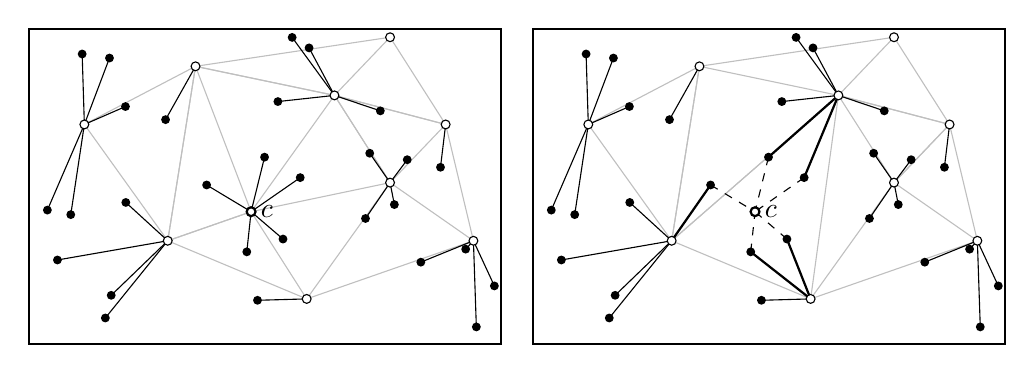
\begin{tikzpicture}[scale=0.4]

\draw [<->,thick] (0,0) rectangle (15,10) {};
\draw [-,gray!50] (11.471,5.115) -- (8.824,1.423);
\draw [-,gray!50] (9.706,7.885) -- (5.294,8.808);
\draw [-,gray!50] (11.471,5.115) -- (7.059,4.192);
\draw [-,gray!50] (13.235,6.962) -- (11.471,5.115);
\draw [-,gray!50] (7.059,4.192) -- (4.412,3.269);
\draw [-,gray!50] (4.412,3.269) -- (7.059,4.192);
\draw [-,gray!50] (11.471,5.115) -- (14.118,3.269);
\draw [-,gray!50] (13.235,6.962) -- (11.471,9.731);
\draw [-,gray!50] (5.294,8.808) -- (1.765,6.962);
\draw [-,gray!50] (13.235,6.962) -- (14.118,3.269);
\draw [-,gray!50] (5.294,8.808) -- (7.059,4.192);
\draw [-,gray!50] (5.294,8.808) -- (4.412,3.269);
\draw [-,gray!50] (8.824,1.423) -- (14.118,3.269);
\draw [-,gray!50] (5.294,8.808) -- (11.471,9.731);
\draw [-,gray!50] (13.235,6.962) -- (9.706,7.885);
\draw [-,gray!50] (9.706,7.885) -- (11.471,5.115);
\draw [-,gray!50] (4.412,3.269) -- (8.824,1.423);
\draw [-,gray!50] (4.412,3.269) -- (1.765,6.962);
\draw [-,gray!50] (4.412,3.269) -- (5.294,8.808);
\draw [-,gray!50] (9.706,7.885) -- (11.471,9.731);
\draw [-,gray!50] (9.706,7.885) -- (7.059,4.192);
\draw [-,gray!50] (11.471,5.115) -- (9.706,7.885);
\draw [-,gray!50] (9.706,7.885) -- (13.235,6.962);
\draw [-,gray!50] (7.059,4.192) -- (8.824,1.423);
\draw [-,gray!50] (5.294,8.808) -- (9.706,7.885);
\draw [-](7.261764705882353, 1.3796923076923076) -- (8.823529411764707, 1.4230769230769231);
\draw [-](10.690588235294118, 3.9763076923076923) -- (11.470588235294118, 5.115384615384615);
\draw [-](3.0697058823529413, 7.531076923076923) -- (1.7647058823529411, 6.961538461538462);
\draw [-](11.161764705882353, 7.393538461538461) -- (9.705882352941176, 7.884615384615385);
\draw [-](2.4308823529411763, 0.8175384615384615) -- (4.411764705882353, 3.269230769230769);
\draw [-](11.60735294117647, 4.418461538461538) -- (11.470588235294118, 5.115384615384615);
\draw [-](2.617058823529412, 1.5375384615384617) -- (4.411764705882353, 3.269230769230769);
\draw [-](0.5902941176470589, 4.243076923076923) -- (1.7647058823529411, 6.961538461538462);
\draw [-](1.695, 9.199076923076923) -- (1.7647058823529411, 6.961538461538462);
\draw [-](4.342941176470588, 7.114769230769231) -- (5.294117647058823, 8.807692307692308);
\draw [-](8.899411764705881, 9.392923076923077) -- (9.705882352941176, 7.884615384615385);
\draw [-](14.21029411764706, 0.5341538461538462) -- (14.117647058823529, 3.269230769230769);
\draw [-](14.78294117647059, 1.8356923076923077) -- (14.117647058823529, 3.269230769230769);
\draw [-](13.871470588235294, 3.0033846153846158) -- (14.117647058823529, 3.269230769230769);
\draw [-](1.333235294117647, 4.099076923076923) -- (1.7647058823529411, 6.961538461538462);
\draw [-](2.5623529411764707, 9.070769230769232) -- (1.7647058823529411, 6.961538461538462);
\draw [-](12.015882352941176, 5.842769230769231) -- (11.470588235294118, 5.115384615384615);
\draw [-](12.448235294117648, 2.5898461538461537) -- (14.117647058823529, 3.269230769230769);
\draw [-](0.909705882352941, 2.659076923076923) -- (4.411764705882353, 3.269230769230769);
\draw [-](3.0811764705882356, 4.485846153846154) -- (4.411764705882353, 3.269230769230769);
\draw [-](8.362058823529411, 9.726153846153846) -- (9.705882352941176, 7.884615384615385);
\draw [-](10.824705882352943, 6.048615384615385) -- (11.470588235294118, 5.115384615384615);
\draw [-](13.072058823529412, 5.602769230769231) -- (13.235294117647058, 6.961538461538462);
\draw [-](7.909411764705883, 7.688923076923077) -- (9.705882352941176, 7.884615384615385);
\draw [-](8.617941176470588, 5.274153846153846) -- (7.0588235294117645, 4.1923076923076925);
\draw [-](7.485882352941177, 5.924) -- (7.0588235294117645, 4.1923076923076925);
\draw [-](5.647058823529412, 5.040615384615384) -- (7.0588235294117645, 4.1923076923076925);
\draw [-](8.071764705882353, 3.3236923076923075) -- (7.0588235294117645, 4.1923076923076925);
\draw [-](6.922058823529412, 2.917538461538462) -- (7.0588235294117645, 4.1923076923076925);
\fill [white](1.7647058823529411, 6.961538461538462)circle(4pt);
\draw (1.7647058823529411, 6.961538461538462)circle(4pt);
\fill [white](4.411764705882353, 3.269230769230769)circle(4pt);
\draw (4.411764705882353, 3.269230769230769)circle(4pt);
\fill [white](5.294117647058823, 8.807692307692308)circle(4pt);
\draw (5.294117647058823, 8.807692307692308)circle(4pt);
\fill [white](8.823529411764707, 1.4230769230769231)circle(4pt);
\draw (8.823529411764707, 1.4230769230769231)circle(4pt);
\fill [white](9.705882352941176, 7.884615384615385)circle(4pt);
\draw (9.705882352941176, 7.884615384615385)circle(4pt);
\fill [white](11.470588235294118, 5.115384615384615)circle(4pt);
\draw (11.470588235294118, 5.115384615384615)circle(4pt);
\fill [white](11.470588235294118, 9.73076923076923)circle(4pt);
\draw (11.470588235294118, 9.73076923076923)circle(4pt);
\fill [white](13.235294117647058, 6.961538461538462)circle(4pt);
\draw (13.235294117647058, 6.961538461538462)circle(4pt);
\fill [white](14.117647058823529, 3.269230769230769)circle(4pt);
\draw (14.117647058823529, 3.269230769230769)circle(4pt);
\fill [white](7.0588235294117645, 4.1923076923076925)circle(4pt);
\draw [thick](7.0588235294117645, 4.1923076923076925)circle(4pt);
\fill(7.261764705882353, 1.3796923076923076)circle(4pt);
\fill(10.690588235294118, 3.9763076923076923)circle(4pt);
\fill(3.0697058823529413, 7.531076923076923)circle(4pt);
\fill(11.161764705882353, 7.393538461538461)circle(4pt);
\fill(2.4308823529411763, 0.8175384615384615)circle(4pt);
\fill(11.60735294117647, 4.418461538461538)circle(4pt);
\fill(2.617058823529412, 1.5375384615384617)circle(4pt);
\fill(8.617941176470588, 5.274153846153846)circle(4pt);
\fill(0.5902941176470589, 4.243076923076923)circle(4pt);
\fill(1.695, 9.199076923076923)circle(4pt);
\fill(4.342941176470588, 7.114769230769231)circle(4pt);
\fill(8.899411764705881, 9.392923076923077)circle(4pt);
\fill(7.485882352941177, 5.924)circle(4pt);
\fill(14.21029411764706, 0.5341538461538462)circle(4pt);
\fill(14.78294117647059, 1.8356923076923077)circle(4pt);
\fill(13.871470588235294, 3.0033846153846158)circle(4pt);
\fill(1.333235294117647, 4.099076923076923)circle(4pt);
\fill(2.5623529411764707, 9.070769230769232)circle(4pt);
\fill(12.015882352941176, 5.842769230769231)circle(4pt);
\fill(12.448235294117648, 2.5898461538461537)circle(4pt);
\fill(0.909705882352941, 2.659076923076923)circle(4pt);
\fill(3.0811764705882356, 4.485846153846154)circle(4pt);
\fill(8.362058823529411, 9.726153846153846)circle(4pt);
\fill(10.824705882352943, 6.048615384615385)circle(4pt);
\fill(5.647058823529412, 5.040615384615384)circle(4pt);
\fill(8.071764705882353, 3.3236923076923075)circle(4pt);
\fill(13.072058823529412, 5.602769230769231)circle(4pt);
\fill(6.922058823529412, 2.917538461538462)circle(4pt);
\fill(7.909411764705883, 7.688923076923077)circle(4pt);
\node at (7.0588235294117645, 4.1923076923076925)[right] {$c$};
\begin{scope}[shift={(16,0)}]
\draw [<->,thick] (0,0) rectangle (15,10) {};
\draw [-,gray!50] (11.471,5.115) -- (8.824,1.423);
\draw [-,gray!50] (13.235,6.962) -- (11.471,5.115);
\draw [-,gray!50] (13.235,6.962) -- (11.471,9.731);
\draw [-,gray!50] (9.706,7.885) -- (4.412,3.269);
\draw [-,gray!50] (11.471,5.115) -- (14.118,3.269);
\draw [-,gray!50] (5.294,8.808) -- (1.765,6.962);
\draw [-,gray!50] (11.471,5.115) -- (13.235,6.962);
\draw [-,gray!50] (5.294,8.808) -- (4.412,3.269);
\draw [-,gray!50] (8.824,1.423) -- (14.118,3.269);
\draw [-,gray!50] (5.294,8.808) -- (11.471,9.731);
\draw [-,gray!50] (13.235,6.962) -- (9.706,7.885);
\draw [-,gray!50] (4.412,3.269) -- (8.824,1.423);
\draw [-,gray!50] (4.412,3.269) -- (1.765,6.962);
\draw [-,gray!50] (4.412,3.269) -- (5.294,8.808);
\draw [-,gray!50] (9.706,7.885) -- (11.471,9.731);
\draw [-,gray!50] (9.706,7.885) -- (8.824,1.423);
\draw [-,gray!50] (4.412,3.269) -- (9.706,7.885);
\draw [-,gray!50] (11.471,5.115) -- (9.706,7.885);
\draw [-,gray!50] (9.706,7.885) -- (13.235,6.962);
\draw [-,gray!50] (13.235,6.962) -- (14.118,3.269);
\draw [-,gray!50] (5.294,8.808) -- (9.706,7.885);
\draw [-](7.261764705882353, 1.3796923076923076) -- (8.823529411764707, 1.4230769230769231);
\draw [-](10.690588235294118, 3.9763076923076923) -- (11.470588235294118, 5.115384615384615);
\draw [-](3.0697058823529413, 7.531076923076923) -- (1.7647058823529411, 6.961538461538462);
\draw [-](11.161764705882353, 7.393538461538461) -- (9.705882352941176, 7.884615384615385);
\draw [-](2.4308823529411763, 0.8175384615384615) -- (4.411764705882353, 3.269230769230769);
\draw [-](11.60735294117647, 4.418461538461538) -- (11.470588235294118, 5.115384615384615);
\draw [-](2.617058823529412, 1.5375384615384617) -- (4.411764705882353, 3.269230769230769);
\draw [-,thick](8.617941176470588, 5.274153846153846) -- (9.705882352941176, 7.884615384615385);
\draw [-](0.5902941176470589, 4.243076923076923) -- (1.7647058823529411, 6.961538461538462);
\draw [-](1.695, 9.199076923076923) -- (1.7647058823529411, 6.961538461538462);
\draw [-](4.342941176470588, 7.114769230769231) -- (5.294117647058823, 8.807692307692308);
\draw [-](8.899411764705881, 9.392923076923077) -- (9.705882352941176, 7.884615384615385);
\draw [-,thick](7.485882352941177, 5.924) -- (9.705882352941176, 7.884615384615385);
\draw [-](14.21029411764706, 0.5341538461538462) -- (14.117647058823529, 3.269230769230769);
\draw [-](14.78294117647059, 1.8356923076923077) -- (14.117647058823529, 3.269230769230769);
\draw [-](13.871470588235294, 3.0033846153846158) -- (14.117647058823529, 3.269230769230769);
\draw [-](1.333235294117647, 4.099076923076923) -- (1.7647058823529411, 6.961538461538462);
\draw [-](2.5623529411764707, 9.070769230769232) -- (1.7647058823529411, 6.961538461538462);
\draw [-](12.015882352941176, 5.842769230769231) -- (11.470588235294118, 5.115384615384615);
\draw [-](12.448235294117648, 2.5898461538461537) -- (14.117647058823529, 3.269230769230769);
\draw [-](0.909705882352941, 2.659076923076923) -- (4.411764705882353, 3.269230769230769);
\draw [-](3.0811764705882356, 4.485846153846154) -- (4.411764705882353, 3.269230769230769);
\draw [-](8.362058823529411, 9.726153846153846) -- (9.705882352941176, 7.884615384615385);
\draw [-](10.824705882352943, 6.048615384615385) -- (11.470588235294118, 5.115384615384615);
\draw [-,thick](5.647058823529412, 5.040615384615384) -- (4.411764705882353, 3.269230769230769);
\draw [-,thick](8.071764705882353, 3.3236923076923075) -- (8.823529411764707, 1.4230769230769231);
\draw [-](13.072058823529412, 5.602769230769231) -- (13.235294117647058, 6.961538461538462);
\draw [-,thick](6.922058823529412, 2.917538461538462) -- (8.823529411764707, 1.4230769230769231);
\draw [-](7.909411764705883, 7.688923076923077) -- (9.705882352941176, 7.884615384615385);
\draw [-,dashed](8.617941176470588, 5.274153846153846) -- (7.0588235294117645, 4.1923076923076925);
\draw [-,dashed](7.485882352941177, 5.924) -- (7.0588235294117645, 4.1923076923076925);
\draw [-,dashed](5.647058823529412, 5.040615384615384) -- (7.0588235294117645, 4.1923076923076925);
\draw [-,dashed](8.071764705882353, 3.3236923076923075) -- (7.0588235294117645, 4.1923076923076925);
\draw [-,dashed](6.922058823529412, 2.917538461538462) -- (7.0588235294117645, 4.1923076923076925);
\fill [white](1.7647058823529411, 6.961538461538462)circle(4pt);
\draw (1.7647058823529411, 6.961538461538462)circle(4pt);
\fill [white](4.411764705882353, 3.269230769230769)circle(4pt);
\draw (4.411764705882353, 3.269230769230769)circle(4pt);
\fill [white](5.294117647058823, 8.807692307692308)circle(4pt);
\draw (5.294117647058823, 8.807692307692308)circle(4pt);
\fill [white](8.823529411764707, 1.4230769230769231)circle(4pt);
\draw (8.823529411764707, 1.4230769230769231)circle(4pt);
\fill [white](9.705882352941176, 7.884615384615385)circle(4pt);
\draw (9.705882352941176, 7.884615384615385)circle(4pt);
\fill [white](11.470588235294118, 5.115384615384615)circle(4pt);
\draw (11.470588235294118, 5.115384615384615)circle(4pt);
\fill [white](11.470588235294118, 9.73076923076923)circle(4pt);
\draw (11.470588235294118, 9.73076923076923)circle(4pt);
\fill [white](13.235294117647058, 6.961538461538462)circle(4pt);
\draw (13.235294117647058, 6.961538461538462)circle(4pt);
\fill [white](14.117647058823529, 3.269230769230769)circle(4pt);
\draw (14.117647058823529, 3.269230769230769)circle(4pt);
\fill [white](7.0588235294117645, 4.1923076923076925)circle(4pt);
\draw [thick](7.0588235294117645, 4.1923076923076925)circle(4pt);
\fill(7.261764705882353, 1.3796923076923076)circle(4pt);
\fill(10.690588235294118, 3.9763076923076923)circle(4pt);
\fill(3.0697058823529413, 7.531076923076923)circle(4pt);
\fill(11.161764705882353, 7.393538461538461)circle(4pt);
\fill(2.4308823529411763, 0.8175384615384615)circle(4pt);
\fill(11.60735294117647, 4.418461538461538)circle(4pt);
\fill(2.617058823529412, 1.5375384615384617)circle(4pt);
\fill(8.617941176470588, 5.274153846153846)circle(4pt);
\fill(0.5902941176470589, 4.243076923076923)circle(4pt);
\fill(1.695, 9.199076923076923)circle(4pt);
\fill(4.342941176470588, 7.114769230769231)circle(4pt);
\fill(8.899411764705881, 9.392923076923077)circle(4pt);
\fill(7.485882352941177, 5.924)circle(4pt);
\fill(14.21029411764706, 0.5341538461538462)circle(4pt);
\fill(14.78294117647059, 1.8356923076923077)circle(4pt);
\fill(13.871470588235294, 3.0033846153846158)circle(4pt);
\fill(1.333235294117647, 4.099076923076923)circle(4pt);
\fill(2.5623529411764707, 9.070769230769232)circle(4pt);
\fill(12.015882352941176, 5.842769230769231)circle(4pt);
\fill(12.448235294117648, 2.5898461538461537)circle(4pt);
\fill(0.909705882352941, 2.659076923076923)circle(4pt);
\fill(3.0811764705882356, 4.485846153846154)circle(4pt);
\fill(8.362058823529411, 9.726153846153846)circle(4pt);
\fill(10.824705882352943, 6.048615384615385)circle(4pt);
\fill(5.647058823529412, 5.040615384615384)circle(4pt);
\fill(8.071764705882353, 3.3236923076923075)circle(4pt);
\fill(13.072058823529412, 5.602769230769231)circle(4pt);
\fill(6.922058823529412, 2.917538461538462)circle(4pt);
\fill(7.909411764705883, 7.688923076923077)circle(4pt);
\node at (7.0588235294117645, 4.1923076923076925)[right] {$c$};
\end{scope}
\end{tikzpicture}
\caption[Illustration of a centroid removal using the geometric method]{Illustration of a centroid removal using the geometric method. This operation is done by retrieving the previous state of the triangulation. Only the points covered by neighbour points of the removed centroid $c$ need to be considered for the assignment update.}
\label{fig:grcent}
\end{figure}


\paragraph{Removing a Non-Centroid}
Removing a non-centroid $n$ only requires recovering the second farthest point if $n$ is currently the farthest point, otherwise, no operations besides erasing $n$'s assignment, taking $\mathcal{O}(1)$ time and memory. Figure \ref{fig:grncent} illustrates this operation.

\begin{figure}[H]
\centering
\begin{minipage}{0.45\linewidth}
\centering
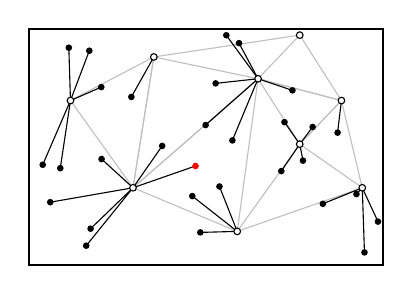
\begin{tikzpicture}[scale=0.3]

\draw [<->,thick] (0,0) rectangle (15,10) {};
\draw [-,gray!50] (11.471,5.115) -- (8.824,1.423);
\draw [-,gray!50] (13.235,6.962) -- (11.471,5.115);
\draw [-,gray!50] (13.235,6.962) -- (11.471,9.731);
\draw [-,gray!50] (9.706,7.885) -- (4.412,3.269);
\draw [-,gray!50] (11.471,5.115) -- (14.118,3.269);
\draw [-,gray!50] (5.294,8.808) -- (1.765,6.962);
\draw [-,gray!50] (11.471,5.115) -- (13.235,6.962);
\draw [-,gray!50] (5.294,8.808) -- (4.412,3.269);
\draw [-,gray!50] (8.824,1.423) -- (14.118,3.269);
\draw [-,gray!50] (5.294,8.808) -- (11.471,9.731);
\draw [-,gray!50] (13.235,6.962) -- (9.706,7.885);
\draw [-,gray!50] (4.412,3.269) -- (8.824,1.423);
\draw [-,gray!50] (4.412,3.269) -- (1.765,6.962);
\draw [-,gray!50] (4.412,3.269) -- (5.294,8.808);
\draw [-,gray!50] (9.706,7.885) -- (11.471,9.731);
\draw [-,gray!50] (9.706,7.885) -- (8.824,1.423);
\draw [-,gray!50] (4.412,3.269) -- (9.706,7.885);
\draw [-,gray!50] (11.471,5.115) -- (9.706,7.885);
\draw [-,gray!50] (9.706,7.885) -- (13.235,6.962);
\draw [-,gray!50] (13.235,6.962) -- (14.118,3.269);
\draw [-,gray!50] (5.294,8.808) -- (9.706,7.885);
\draw [-](7.261764705882353, 1.3796923076923076) -- (8.823529411764707, 1.4230769230769231);
\draw [-](10.690588235294118, 3.9763076923076923) -- (11.470588235294118, 5.115384615384615);
\draw [-](3.0697058823529413, 7.531076923076923) -- (1.7647058823529411, 6.961538461538462);
\draw [-](11.161764705882353, 7.393538461538461) -- (9.705882352941176, 7.884615384615385);
\draw [-](2.4308823529411763, 0.8175384615384615) -- (4.411764705882353, 3.269230769230769);
\draw [-](11.60735294117647, 4.418461538461538) -- (11.470588235294118, 5.115384615384615);
\draw [-](2.617058823529412, 1.5375384615384617) -- (4.411764705882353, 3.269230769230769);
\draw [-](8.617941176470588, 5.274153846153846) -- (9.705882352941176, 7.884615384615385);
\draw [-](0.5902941176470589, 4.243076923076923) -- (1.7647058823529411, 6.961538461538462);
\draw [-](1.695, 9.199076923076923) -- (1.7647058823529411, 6.961538461538462);
\draw [-](4.342941176470588, 7.114769230769231) -- (5.294117647058823, 8.807692307692308);
\draw [-](8.899411764705881, 9.392923076923077) -- (9.705882352941176, 7.884615384615385);
\draw [-](7.485882352941177, 5.924) -- (9.705882352941176, 7.884615384615385);
\draw [-](14.21029411764706, 0.5341538461538462) -- (14.117647058823529, 3.269230769230769);
\draw [-](14.78294117647059, 1.8356923076923077) -- (14.117647058823529, 3.269230769230769);
\draw [-](13.871470588235294, 3.0033846153846158) -- (14.117647058823529, 3.269230769230769);
\draw [-](1.333235294117647, 4.099076923076923) -- (1.7647058823529411, 6.961538461538462);
\draw [-](2.5623529411764707, 9.070769230769232) -- (1.7647058823529411, 6.961538461538462);
\draw [-](12.015882352941176, 5.842769230769231) -- (11.470588235294118, 5.115384615384615);
\draw [-](12.448235294117648, 2.5898461538461537) -- (14.117647058823529, 3.269230769230769);
\draw [-](0.909705882352941, 2.659076923076923) -- (4.411764705882353, 3.269230769230769);
\draw [-](3.0811764705882356, 4.485846153846154) -- (4.411764705882353, 3.269230769230769);
\draw [-](8.362058823529411, 9.726153846153846) -- (9.705882352941176, 7.884615384615385);
\draw [-](10.824705882352943, 6.048615384615385) -- (11.470588235294118, 5.115384615384615);
\draw [-](5.647058823529412, 5.040615384615384) -- (4.411764705882353, 3.269230769230769);
\draw [-](8.071764705882353, 3.3236923076923075) -- (8.823529411764707, 1.4230769230769231);
\draw [-](13.072058823529412, 5.602769230769231) -- (13.235294117647058, 6.961538461538462);
\draw [-](6.922058823529412, 2.917538461538462) -- (8.823529411764707, 1.4230769230769231);
\draw [-](7.909411764705883, 7.688923076923077) -- (9.705882352941176, 7.884615384615385);
\draw [-](7.0588235294117645, 4.1923076923076925) -- (4.411764705882353, 3.269230769230769);
\fill [white](1.7647058823529411, 6.961538461538462)circle(4pt);
\draw (1.7647058823529411, 6.961538461538462)circle(4pt);
\fill [white](4.411764705882353, 3.269230769230769)circle(4pt);
\draw (4.411764705882353, 3.269230769230769)circle(4pt);
\fill [white](5.294117647058823, 8.807692307692308)circle(4pt);
\draw (5.294117647058823, 8.807692307692308)circle(4pt);
\fill [white](8.823529411764707, 1.4230769230769231)circle(4pt);
\draw (8.823529411764707, 1.4230769230769231)circle(4pt);
\fill [white](9.705882352941176, 7.884615384615385)circle(4pt);
\draw (9.705882352941176, 7.884615384615385)circle(4pt);
\fill [white](11.470588235294118, 5.115384615384615)circle(4pt);
\draw (11.470588235294118, 5.115384615384615)circle(4pt);
\fill [white](11.470588235294118, 9.73076923076923)circle(4pt);
\draw (11.470588235294118, 9.73076923076923)circle(4pt);
\fill [white](13.235294117647058, 6.961538461538462)circle(4pt);
\draw (13.235294117647058, 6.961538461538462)circle(4pt);
\fill [white](14.117647058823529, 3.269230769230769)circle(4pt);
\draw (14.117647058823529, 3.269230769230769)circle(4pt);
\fill [red](7.0588235294117645, 4.1923076923076925)circle(4pt);
\fill(7.261764705882353, 1.3796923076923076)circle(4pt);
\fill(10.690588235294118, 3.9763076923076923)circle(4pt);
\fill(3.0697058823529413, 7.531076923076923)circle(4pt);
\fill(11.161764705882353, 7.393538461538461)circle(4pt);
\fill(2.4308823529411763, 0.8175384615384615)circle(4pt);
\fill(11.60735294117647, 4.418461538461538)circle(4pt);
\fill(2.617058823529412, 1.5375384615384617)circle(4pt);
\fill(8.617941176470588, 5.274153846153846)circle(4pt);
\fill(0.5902941176470589, 4.243076923076923)circle(4pt);
\fill(1.695, 9.199076923076923)circle(4pt);
\fill(4.342941176470588, 7.114769230769231)circle(4pt);
\fill(8.899411764705881, 9.392923076923077)circle(4pt);
\fill(7.485882352941177, 5.924)circle(4pt);
\fill(14.21029411764706, 0.5341538461538462)circle(4pt);
\fill(14.78294117647059, 1.8356923076923077)circle(4pt);
\fill(13.871470588235294, 3.0033846153846158)circle(4pt);
\fill(1.333235294117647, 4.099076923076923)circle(4pt);
\fill(2.5623529411764707, 9.070769230769232)circle(4pt);
\fill(12.015882352941176, 5.842769230769231)circle(4pt);
\fill(12.448235294117648, 2.5898461538461537)circle(4pt);
\fill(0.909705882352941, 2.659076923076923)circle(4pt);
\fill(3.0811764705882356, 4.485846153846154)circle(4pt);
\fill(8.362058823529411, 9.726153846153846)circle(4pt);
\fill(10.824705882352943, 6.048615384615385)circle(4pt);
\fill(5.647058823529412, 5.040615384615384)circle(4pt);
\fill(8.071764705882353, 3.3236923076923075)circle(4pt);
\fill(13.072058823529412, 5.602769230769231)circle(4pt);
\fill(6.922058823529412, 2.917538461538462)circle(4pt);
\fill(7.909411764705883, 7.688923076923077)circle(4pt);
\end{tikzpicture}\end{minipage}\begin{minipage}{0.45\linewidth}\centering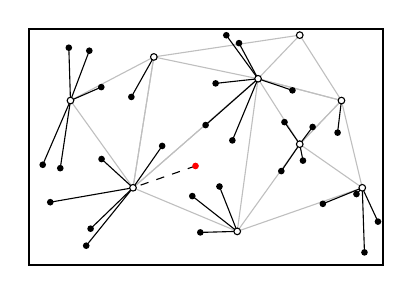
\begin{tikzpicture}[scale=0.3]
\draw [<->,thick] (0,0) rectangle (15,10) {};
\draw [-,gray!50] (11.471,5.115) -- (8.824,1.423);
\draw [-,gray!50] (13.235,6.962) -- (11.471,5.115);
\draw [-,gray!50] (13.235,6.962) -- (11.471,9.731);
\draw [-,gray!50] (9.706,7.885) -- (4.412,3.269);
\draw [-,gray!50] (11.471,5.115) -- (14.118,3.269);
\draw [-,gray!50] (5.294,8.808) -- (1.765,6.962);
\draw [-,gray!50] (11.471,5.115) -- (13.235,6.962);
\draw [-,gray!50] (5.294,8.808) -- (4.412,3.269);
\draw [-,gray!50] (8.824,1.423) -- (14.118,3.269);
\draw [-,gray!50] (5.294,8.808) -- (11.471,9.731);
\draw [-,gray!50] (13.235,6.962) -- (9.706,7.885);
\draw [-,gray!50] (4.412,3.269) -- (8.824,1.423);
\draw [-,gray!50] (4.412,3.269) -- (1.765,6.962);
\draw [-,gray!50] (4.412,3.269) -- (5.294,8.808);
\draw [-,gray!50] (9.706,7.885) -- (11.471,9.731);
\draw [-,gray!50] (9.706,7.885) -- (8.824,1.423);
\draw [-,gray!50] (4.412,3.269) -- (9.706,7.885);
\draw [-,gray!50] (11.471,5.115) -- (9.706,7.885);
\draw [-,gray!50] (9.706,7.885) -- (13.235,6.962);
\draw [-,gray!50] (13.235,6.962) -- (14.118,3.269);
\draw [-,gray!50] (5.294,8.808) -- (9.706,7.885);
\draw [-](7.261764705882353, 1.3796923076923076) -- (8.823529411764707, 1.4230769230769231);
\draw [-](10.690588235294118, 3.9763076923076923) -- (11.470588235294118, 5.115384615384615);
\draw [-](3.0697058823529413, 7.531076923076923) -- (1.7647058823529411, 6.961538461538462);
\draw [-](11.161764705882353, 7.393538461538461) -- (9.705882352941176, 7.884615384615385);
\draw [-](2.4308823529411763, 0.8175384615384615) -- (4.411764705882353, 3.269230769230769);
\draw [-](11.60735294117647, 4.418461538461538) -- (11.470588235294118, 5.115384615384615);
\draw [-](2.617058823529412, 1.5375384615384617) -- (4.411764705882353, 3.269230769230769);
\draw [-](8.617941176470588, 5.274153846153846) -- (9.705882352941176, 7.884615384615385);
\draw [-](0.5902941176470589, 4.243076923076923) -- (1.7647058823529411, 6.961538461538462);
\draw [-](1.695, 9.199076923076923) -- (1.7647058823529411, 6.961538461538462);
\draw [-](4.342941176470588, 7.114769230769231) -- (5.294117647058823, 8.807692307692308);
\draw [-](8.899411764705881, 9.392923076923077) -- (9.705882352941176, 7.884615384615385);
\draw [-](7.485882352941177, 5.924) -- (9.705882352941176, 7.884615384615385);
\draw [-](14.21029411764706, 0.5341538461538462) -- (14.117647058823529, 3.269230769230769);
\draw [-](14.78294117647059, 1.8356923076923077) -- (14.117647058823529, 3.269230769230769);
\draw [-](13.871470588235294, 3.0033846153846158) -- (14.117647058823529, 3.269230769230769);
\draw [-](1.333235294117647, 4.099076923076923) -- (1.7647058823529411, 6.961538461538462);
\draw [-](2.5623529411764707, 9.070769230769232) -- (1.7647058823529411, 6.961538461538462);
\draw [-](12.015882352941176, 5.842769230769231) -- (11.470588235294118, 5.115384615384615);
\draw [-](12.448235294117648, 2.5898461538461537) -- (14.117647058823529, 3.269230769230769);
\draw [-](0.909705882352941, 2.659076923076923) -- (4.411764705882353, 3.269230769230769);
\draw [-](3.0811764705882356, 4.485846153846154) -- (4.411764705882353, 3.269230769230769);
\draw [-](8.362058823529411, 9.726153846153846) -- (9.705882352941176, 7.884615384615385);
\draw [-](10.824705882352943, 6.048615384615385) -- (11.470588235294118, 5.115384615384615);
\draw [-](5.647058823529412, 5.040615384615384) -- (4.411764705882353, 3.269230769230769);
\draw [-](8.071764705882353, 3.3236923076923075) -- (8.823529411764707, 1.4230769230769231);
\draw [-](13.072058823529412, 5.602769230769231) -- (13.235294117647058, 6.961538461538462);
\draw [-](6.922058823529412, 2.917538461538462) -- (8.823529411764707, 1.4230769230769231);
\draw [-](7.909411764705883, 7.688923076923077) -- (9.705882352941176, 7.884615384615385);
\draw [-,dashed](7.0588235294117645, 4.1923076923076925) -- (4.411764705882353, 3.269230769230769);
\fill [white](1.7647058823529411, 6.961538461538462)circle(4pt);
\draw (1.7647058823529411, 6.961538461538462)circle(4pt);
\fill [white](4.411764705882353, 3.269230769230769)circle(4pt);
\draw (4.411764705882353, 3.269230769230769)circle(4pt);
\fill [white](5.294117647058823, 8.807692307692308)circle(4pt);
\draw (5.294117647058823, 8.807692307692308)circle(4pt);
\fill [white](8.823529411764707, 1.4230769230769231)circle(4pt);
\draw (8.823529411764707, 1.4230769230769231)circle(4pt);
\fill [white](9.705882352941176, 7.884615384615385)circle(4pt);
\draw (9.705882352941176, 7.884615384615385)circle(4pt);
\fill [white](11.470588235294118, 5.115384615384615)circle(4pt);
\draw (11.470588235294118, 5.115384615384615)circle(4pt);
\fill [white](11.470588235294118, 9.73076923076923)circle(4pt);
\draw (11.470588235294118, 9.73076923076923)circle(4pt);
\fill [white](13.235294117647058, 6.961538461538462)circle(4pt);
\draw (13.235294117647058, 6.961538461538462)circle(4pt);
\fill [white](14.117647058823529, 3.269230769230769)circle(4pt);
\draw (14.117647058823529, 3.269230769230769)circle(4pt);
\fill [red](7.0588235294117645, 4.1923076923076925)circle(4pt);
\fill(7.261764705882353, 1.3796923076923076)circle(4pt);
\fill(10.690588235294118, 3.9763076923076923)circle(4pt);
\fill(3.0697058823529413, 7.531076923076923)circle(4pt);
\fill(11.161764705882353, 7.393538461538461)circle(4pt);
\fill(2.4308823529411763, 0.8175384615384615)circle(4pt);
\fill(11.60735294117647, 4.418461538461538)circle(4pt);
\fill(2.617058823529412, 1.5375384615384617)circle(4pt);
\fill(8.617941176470588, 5.274153846153846)circle(4pt);
\fill(0.5902941176470589, 4.243076923076923)circle(4pt);
\fill(1.695, 9.199076923076923)circle(4pt);
\fill(4.342941176470588, 7.114769230769231)circle(4pt);
\fill(8.899411764705881, 9.392923076923077)circle(4pt);
\fill(7.485882352941177, 5.924)circle(4pt);
\fill(14.21029411764706, 0.5341538461538462)circle(4pt);
\fill(14.78294117647059, 1.8356923076923077)circle(4pt);
\fill(13.871470588235294, 3.0033846153846158)circle(4pt);
\fill(1.333235294117647, 4.099076923076923)circle(4pt);
\fill(2.5623529411764707, 9.070769230769232)circle(4pt);
\fill(12.015882352941176, 5.842769230769231)circle(4pt);
\fill(12.448235294117648, 2.5898461538461537)circle(4pt);
\fill(0.909705882352941, 2.659076923076923)circle(4pt);
\fill(3.0811764705882356, 4.485846153846154)circle(4pt);
\fill(8.362058823529411, 9.726153846153846)circle(4pt);
\fill(10.824705882352943, 6.048615384615385)circle(4pt);
\fill(5.647058823529412, 5.040615384615384)circle(4pt);
\fill(8.071764705882353, 3.3236923076923075)circle(4pt);
\fill(13.072058823529412, 5.602769230769231)circle(4pt);
\fill(6.922058823529412, 2.917538461538462)circle(4pt);
\fill(7.909411764705883, 7.688923076923077)circle(4pt);
\end{tikzpicture}\end{minipage}\end{figure}


\paragraph{Bounds}
The same lower bound described in Section \ref{sec:bounds} can be applied in this approach. Both algorithms have the same time complexity of $\mathcal{O}(N)$ for computing the bound.

These steps occur at each iteration of the branch-and-bound algorithm, and each is performed potentially $2^N$ times for both approaches.
Despite having the same worst-case time complexity as the branch-and-bound algorithm described in Section \ref{alg:bb}, the expected time complexity for the Delaunay assisted approach is smaller. This approach should have better performance when a large number of centroids are needed.
This is especially true since maintaining a valid Delaunay triangulation through all the centroid permutations, as well as the Hilbert sorting, takes a computing cost. This extra overhead has a negative impact in the performance in the smaller instances of the problem.
\section{Algorithm Comparison}

\subsection{Time Complexity}

Each of the procedures mentioned in the previous Section are performed at each step of the recursive tree. At each step the bound is also calculated, which takes $\mathcal{O}(N)$ time. Table \ref{tab:exptime} shows the time complexities for each procedure in both algorithms. The values presented at the row corresponding to the average case of the Delaunay-assisted algorithm are conjectured and need to be shown in a more formal manner.
\begin{table}[!h]
\begin{center}
\begin{tabular}{|c|c|c|c|c|}
	\hline
	\multirow{2}{*}{Algorithm}	& \multicolumn{2}{c|}{Insert}	& \multicolumn{2}{c|}{Remove}	\\ \cline{2-5}
								& Centroid		& Non-Centroid	& Centroid		& Non-Centroid	\\ \hline
				Naïve BB		& $\Theta(N)$ & $\Theta(K)$ 	& $\Theta(N)$ & $\mathcal{O}(1)$ \\ \hline\hline
				Del. Assisted BB	
				& \multirow{2}{*}{$\mathcal{O}(\log{K}+N/K)$}
				& \multirow{2}{*}{$\mathcal{O}(\sqrt{K})$}
				& \multirow{2}{*}{$\mathcal{O}(N/K)$ }
				& \multirow{2}{*}{$\mathcal{O}(1)$}\\
				Average Case & & & & \\ \hline
		Del. Assisted BB 
				& \multirow{2}{*}{$\mathcal{O}(K+N)$}
				& \multirow{2}{*}{$\mathcal{O}(K)$}	
				& \multirow{2}{*}{$\mathcal{O}(N)$} 
				& \multirow{2}{*}{$\mathcal{O}(1)$}\\ 
				Worst Case 	& & & & \\ \hline
\end{tabular}
	\captionof{table}{Time complexities for the various operations in a uniformly distributed point set}
	\label{tab:exptime}
\end{center}
\end{table}
\subsection{Experimental Results}
\paragraph{}
In this section, we analyse empirically the time spent calculating the solutions to different sizes of the problem. 
\subsubsection*{Methodology and Set-up}
The test cases are sets of uniformly distributed points generated with a fixed seed. Each test was repeated 10 times with different sets of points. The same sets and machine were used to test the three algorithms.

Both branch-and-bound approaches were implemented using \emph{C++} and compiled using \emph{g++ 4.9.2}. The integer linear programming version had the data preprocessed using \emph{python 2.7.9} and was solved using the \emph{GLPK LP/MIP v4.55} solver. The programs were ran on a machine with a Intel i7 Dual-Core, 2GHz processor, with a 8 GB, 1600 MHz memory and Arch Linux 3.14.4 x64 as its operating system.

\subsubsection*{Effect of $N$}

The first test conducted analysed the variance in performance relative to changes in the value of $N$. It was done by changing $N$, with $K$ taking fixed fractional values of $N$. Figure \ref{fig:fixed_k} shows the results of these tests. The measures were taken in seconds and account for the pre-processing steps and the solving time, but not the input reading or output writing times. The tests were stopped at the half-hour mark. 
\begin{figure}[t] 
	\begin{subfigure}[b]{0.4\linewidth}
		\centering
		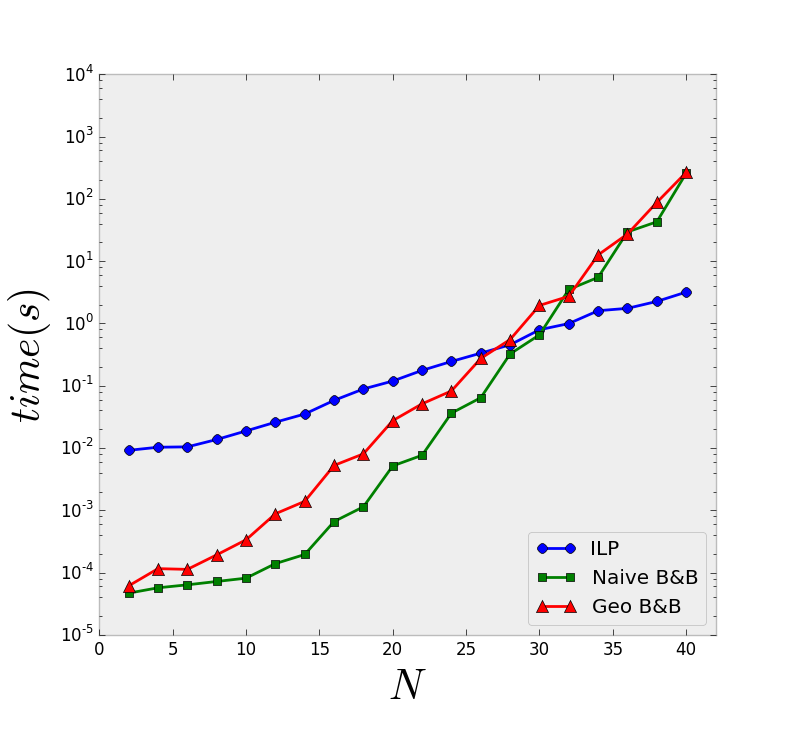
\includegraphics[width=0.9\linewidth]{Pictures/k1} 
		\caption{$K=0.25N$} 
		\label{fig:fixed_k:a} 
	\end{subfigure}%% 
	\begin{subfigure}[b]{0.4\linewidth}
		\centering
		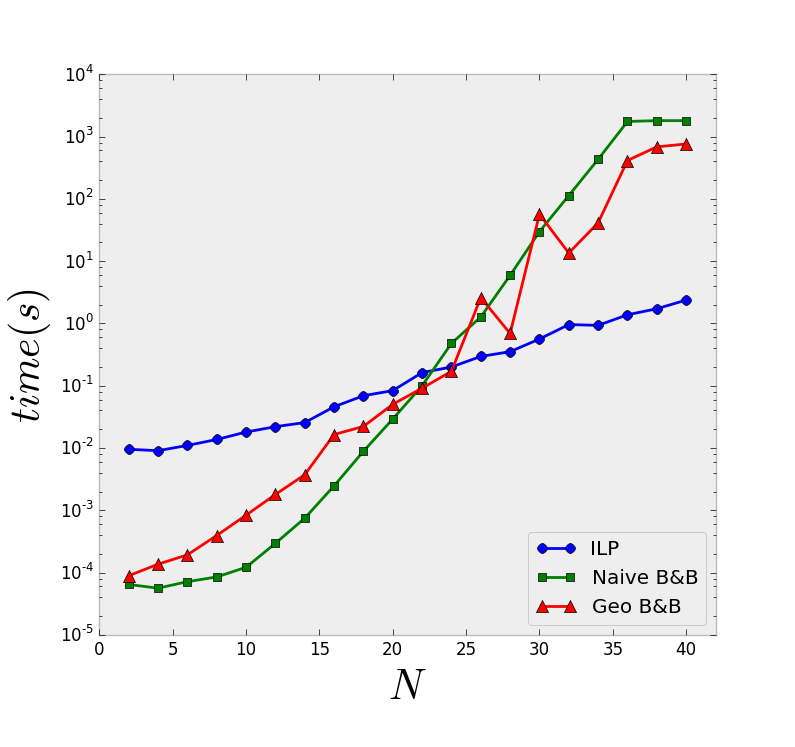
\includegraphics[width=0.9\linewidth]{Pictures/k2} 
		\caption{$K=0.5N$} 
		\label{fig:fixed_k:b} 
	\end{subfigure} 
	\begin{center}
	\begin{subfigure}[b]{0.4\linewidth}
		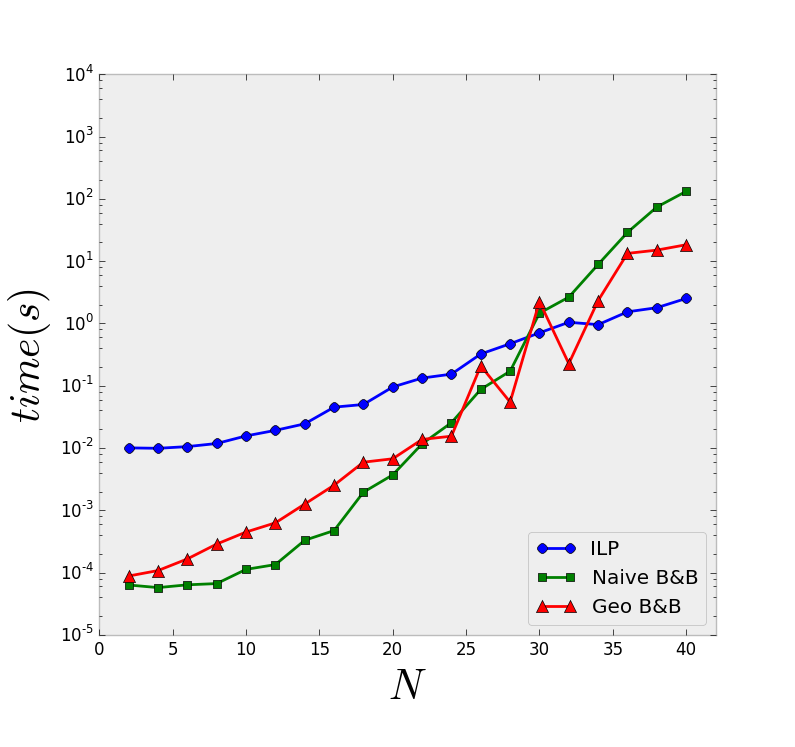
\includegraphics[width=0.9\linewidth]{Pictures/k3} 
		\caption{$K=0.75N$} 
		\label{fig:fixed_k:c} 
	\end{subfigure}
	\end{center}
	\begin{center}
    \textcolor{blue}{\cmark}\ -- Integer Linear Programming\quad   \textcolor{red}{\tmark}\ -- Delaunay Assisted B\&B\quad \textcolor{green}{\smark}\ -- Naive B\&B
    \end{center}
	\caption{CPU-time for different values of $K$ with varying values of $N$}
	\label{fig:fixed_k} 
\end{figure}


\noindent
As it can be seen, the problem solving time increases exponentially with the value of $N$, as expected.
The Integer Linear Programming Approach performs faster for larger values of $N$. Comparing the branch-and-bound approaches, these tests show that the Delaunay-assisted algorithm steadily approaches and surpasses the naïve branch-and-bound algorithm as the instance size grows.
\subsubsection*{Effect of $K$}
In this experiment, we analysed the performance of the three algorithms in dependence of parameter $K$. We fixed $N$ and varied $K$ from 2 to $N$ by steps of 2. Figure \ref{fig:fixed_n} show the results for the $N=\{10,20,30,40\}$, respectively. The tests were stopped at the half-hour mark. Figure \ref{fig:fixed_n} shows the results of these tests.
\begin{figure}[t] 
  \begin{subfigure}[b]{0.5\linewidth}
    \centering
    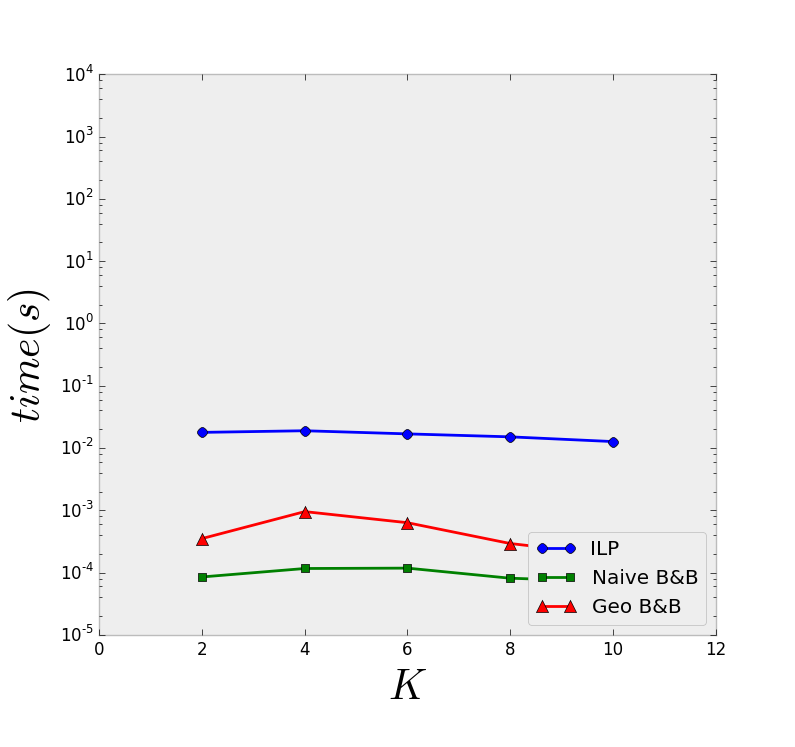
\includegraphics[width=0.9\linewidth]{Pictures/n10} 
    \caption{$N=10$} 
    \label{fig:fixed_n:a} 
    \vspace{4ex}
  \end{subfigure}%% 
  \begin{subfigure}[b]{0.5\linewidth}
    \centering
    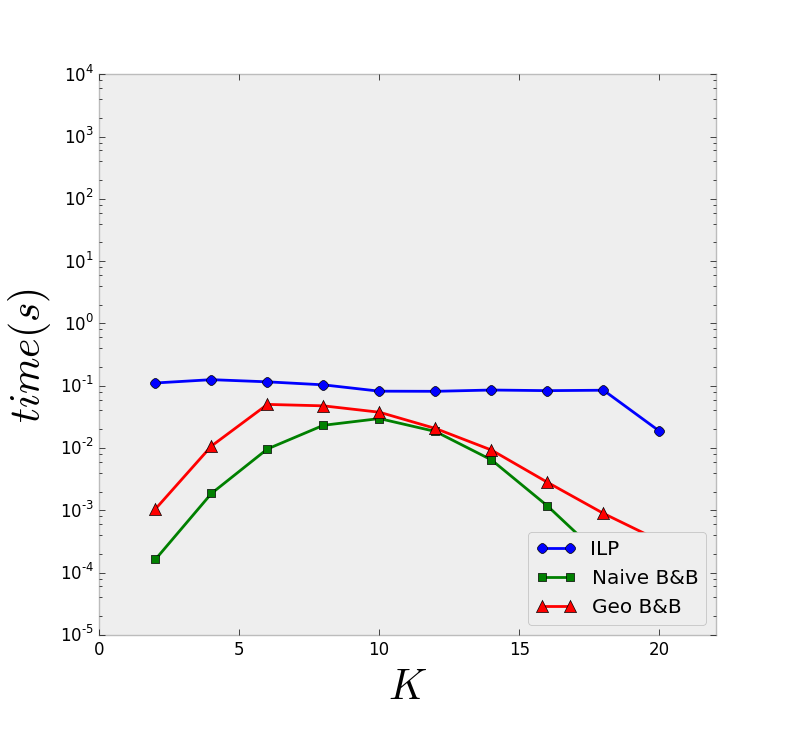
\includegraphics[width=0.9\linewidth]{Pictures/n20} 
    \caption{$N=20$} 
    \label{fig:fixed_n:b} 
    \vspace{4ex}
  \end{subfigure} 
  \begin{subfigure}[b]{0.5\linewidth}
    \centering
    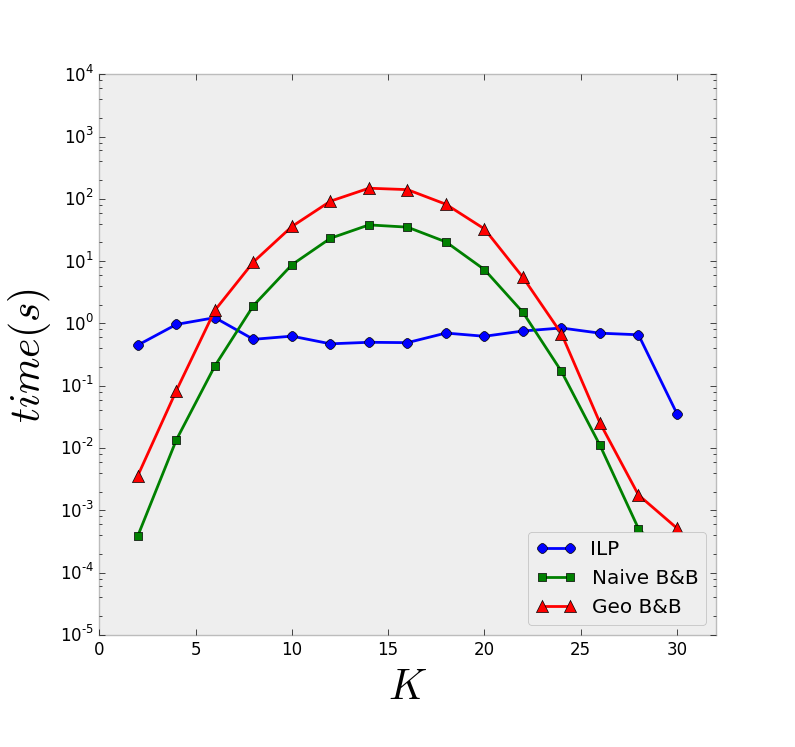
\includegraphics[width=0.9\linewidth]{Pictures/n30} 
    \caption{$N=30$} 
    \label{fig:fixed_n:c} 
  \end{subfigure}%%
  \begin{subfigure}[b]{0.5\linewidth}
    \centering
    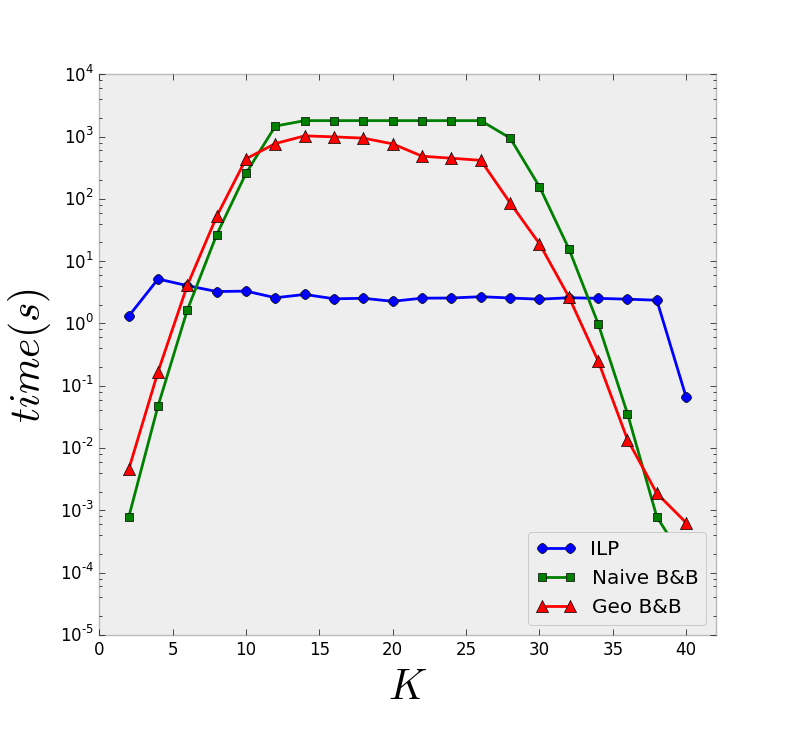
\includegraphics[width=0.9\linewidth]{Pictures/n40} 
    \caption{$N=40$} 
    \label{fig:fixed_n:d} 
  \end{subfigure} 
  \vspace{2ex}
  \begin{center}
  \textcolor{blue}{\cmark}\ -- Integer Linear Programming \quad   \textcolor{red}{\tmark}\ -- Delaunay Assisted B\&B\quad \textcolor{OliveGreen}{\smark}\ -- Naive B\&B
  \end{center}
  \caption{CPU-time for different values of $N$ with varying $K$}
  \label{fig:fixed_n} 
\end{figure}


\noindent
The Integer Linear Programming approach seems to be the fastest approach for most cases, and seems independent to the value of $K$. The exceptions to this seem to be smaller values of $N$, as well as the smallest and largest values of $K$. This happens because the implicit enumeration methods only need to enumerate a very small number of combinations.
As for the branch-and-bound algorithms, the Delaunay-assisted approach is slower than the Naïve implementation in these test cases. However it should be noted that for each $N$, the Delaunay-assisted algorithm peaks before the expected value of $K=N/2$. This is justified due to the fact that the Delaunay triangulation has an overhead which can take advantage for in larger values of $K$.
Furthermore, the fact that the Naïve implementation had no test for the middle values of $K$ for $N=40$ that ended before the time-out mark is noteworthy.
It is also worth noting that The Delaunay-assisted approach showed a lot more variance between tests, often taking much lower values than the mean. However, for the tests performed, two runs had values much larger than the Naïve approach, approximating the Delaunay-assisted algorithm's mean to the Naïve approach.

The time required for each test limited the number of tests performed. Because of this, the results may not be statistically meaningful. 
This could mean that the Delaunay-assisted approach is only preferable for values of $N$ and $K$ to which neither approach is usable in real-time. Due to the small number of tests for large values of $N$, this result may not be statistically meaningful, but it is noteworthy.

\section{Discussion}
The algorithms in this chapter have some drawbacks when used in a web application. Not only were the running times too large to be used in real-time, taking minutes and even hours for small instances with 40 points at most, but they also required some a priori knowledge about the number of clusters on a given window. This is infeasible, since there is no efficient way to infer how many clusters there are in a new region, without testing for all possible values of $K$. The algorithm should be able to calculate the final number of selected points, constrained to a minimum distance factor between them. This can be achieved by solving \emph{Geometric Disk Cover} problem described in Section \ref{ilp2}. The next chapter describes in detail a way to solve this problem in regards to the final application.
